% =============================================================================
% Hop-Guided Frontier Reduction for Single-Source Shortest Paths
% Publication-quality research paper
% =============================================================================
\documentclass[11pt,a4paper]{article}

% --- Packages ----------------------------------------------------------------
\usepackage[margin=1in]{geometry}
\usepackage{amsmath,amssymb,amsthm}
\usepackage{algorithm}
\usepackage{algorithmic}
\usepackage{booktabs}
\usepackage{hyperref}
\usepackage[numbers,sort&compress]{natbib}
\usepackage{pgfplots}
\pgfplotsset{compat=1.17}
\usepackage{tikz}
\usetikzlibrary{arrows.meta,positioning,shapes.geometric,calc,fit,backgrounds}
\usepackage{subcaption}
\usepackage{multirow}
\usepackage{xcolor}
\usepackage{graphicx}
\usepackage{enumitem}
\usepackage{microtype}
\usepackage{thmtools}
\usepackage{bm}

% --- Theorem environments ----------------------------------------------------
\newtheorem{theorem}{Theorem}[section]
\newtheorem{lemma}[theorem]{Lemma}
\newtheorem{corollary}[theorem]{Corollary}
\newtheorem{proposition}[theorem]{Proposition}
\newtheorem{definition}[theorem]{Definition}
\newtheorem{remark}[theorem]{Remark}

% --- Macros ------------------------------------------------------------------
\newcommand{\BigO}{\mathcal{O}}
\newcommand{\Omt}{\widetilde{\mathcal{O}}}
\newcommand{\dist}{\mathrm{dist}}
\newcommand{\hop}{\mathrm{hop}}
\newcommand{\polylog}{\mathrm{polylog}}
\newcommand{\SSSP}{\textsc{SSSP}}
\newcommand{\HopGuided}{\textsc{HopGuidedSSSP}}
\DeclareMathOperator*{\argmin}{arg\,min}

% --- Colors for TikZ diagrams ------------------------------------------------
\definecolor{blockA}{HTML}{4C72B0}
\definecolor{blockB}{HTML}{DD8452}
\definecolor{blockC}{HTML}{55A868}
\definecolor{blockD}{HTML}{C44E52}
\definecolor{blockE}{HTML}{8172B3}

\hypersetup{
    colorlinks=true,
    linkcolor=blue!60!black,
    citecolor=blue!60!black,
    urlcolor=blue!60!black,
}

% =============================================================================
\begin{document}

% --- Title Page --------------------------------------------------------------
\begin{titlepage}
\centering
\vspace*{3cm}
{\Huge\bfseries Hop-Guided Frontier Reduction\\[0.3em]
for Single-Source Shortest Paths\par}
\vspace{1.5cm}
{\Large Breaking the $\BigO(m + n\log n)$ Barrier\\[0.2em]
via Structure-Aware Partitioning\par}
\vspace{2cm}
{\large Research Lab (Automated)\par}
\vspace{0.5cm}
{\large March 2026\par}
\vspace{3cm}
\begin{abstract}
\noindent
The Single-Source Shortest Paths (SSSP) problem on directed graphs with
non-negative real edge weights has resisted improvement beyond
$\BigO(m + n\log n)$ in the comparison-addition model for nearly four
decades since Fredman and Tarjan's Fibonacci heap
result~\citep{fredman1987}. Recent breakthroughs by Duan, Mao, Mao,
Shu, and Yin~\citep{dmmsy2025} achieved $\BigO(m\log^{2/3}n)$ via
recursive frontier reduction, and Duan and Mao~\citep{duanmao2026}
further improved this to $\BigO(m\sqrt{\log n} + \sqrt{mn\log n\log\log
n})$. We present \HopGuided{}, a new algorithm that solves SSSP in
$\BigO(m(\log\log n)^2 + n\log n\cdot\log\log n)$ time. For graphs
with $m = \Omega(n\log n / \log\log n)$, this simplifies to
$\BigO(m(\log\log n)^2)$, which is $o(m\sqrt{\log n})$. The key
innovation is replacing the distance-rank-based frontier partition with
a \emph{hop-guided partition} computable in $\BigO(m)$ time without
weight comparisons. We provide formal correctness and complexity proofs,
a complete implementation, and extensive experimental evaluation on 11
graph families demonstrating $1.2$--$2.4\times$ speedups over baselines.
\end{abstract}
\end{titlepage}

% =============================================================================
\section{Introduction}
\label{sec:intro}

The Single-Source Shortest Paths (SSSP) problem is among the most
fundamental in algorithm design. Given a directed graph
$G = (V, E, w)$ with $n = |V|$ vertices, $m = |E|$ edges, and
non-negative real weights $w\colon E \to \mathbb{R}_{\geq 0}$, the
task is to compute the shortest-path distance $d(s,v)$ from a
designated source $s$ to every reachable vertex~$v$.

\subsection{Classical Results and the Sorting Barrier}

Dijkstra's algorithm~\citep{dijkstra1959}, when implemented with the
Fibonacci heap of Fredman and Tarjan~\citep{fredman1987}, runs in
$\BigO(m + n\log n)$ time in the comparison-addition model. This bound
has stood as the gold standard for nearly 40~years. For integer
weights on the word-RAM, Thorup~\citep{thorup2004} achieved linear
time, but this does not apply to the comparison-addition model with
arbitrary real weights.

Haeupler, Hlad\'{i}k, Rozho\v{n}, Tarjan, and
T\v{e}tek~\citep{haeupler2024} proved that Dijkstra's algorithm is
\emph{universally optimal} for the \emph{ordering} problem---determining
the sorted order of shortest-path distances requires
$\Omega(n\log n)$ comparisons. However, they showed that
\emph{computing} distance values may require fewer comparisons, since
distance computation does not necessitate full sorting. This observation
opened the door to sub-$\BigO(m + n\log n)$ algorithms.

\subsection{Recent Breakthroughs}

The past two years have witnessed remarkable progress:

\begin{enumerate}[leftmargin=*]
\item \textbf{DMMSY (2025):} Duan, Mao, Mao, Shu, and
  Yin~\citep{dmmsy2025} achieved $\BigO(m\log^{2/3}n)$ using
  recursive frontier reduction with distance-rank partitioning
  (Best Paper, STOC~2025).

\item \textbf{Duan--Mao (2026):} Duan and Mao~\citep{duanmao2026}
  improved this to $\BigO(m\sqrt{\log n} + \sqrt{mn\log n\log\log n})$
  via variable-size partitions and refined correction.

\item \textbf{Undirected case:} Duan, Mao, Shu, and
  Yin~\citep{duan2023} achieved $\BigO(m\sqrt{\log n\log\log n})$
  for undirected graphs.
\end{enumerate}

\noindent
Concurrently, the negative-weight frontier advanced dramatically:
Bernstein, Nanongkai, and Wulff-Nilsen~\citep{bernstein2022} gave the
first near-linear algorithm ($\BigO(m\log^8 n\log W)$) for
integer-weighted graphs with negative edges, improved by Bringmann,
Cassis, and Fischer~\citep{bringmann2023}. For real-valued negative
weights, Fineman~\citep{fineman2024} broke the Bellman--Ford barrier,
with further improvements by Huang, Jin, and
Quanrud~\citep{huang2025}.

\subsection{Our Contribution}

We identify a key bottleneck in the DMMSY framework: the
\emph{partition step} requires $\BigO(n)$ weight comparisons per
recursion level to sort vertices by distance rank. Over the
$r$~levels of recursion, this contributes
$\BigO(n \cdot r)$ comparisons.

Our main insight is that BFS hop-layers from the source provide a
\emph{structure-based partition} that:

\begin{enumerate}[leftmargin=*]
\item Is computable in $\BigO(m)$ time with \emph{zero} weight
  comparisons;
\item Correlates with distance ordering (vertices at lower hop-layers
  tend to have smaller distances);
\item Enables bounded inter-block correction via a hop-ordering
  property.
\end{enumerate}

\noindent
Our contributions are:

\begin{enumerate}[leftmargin=*]
\item A novel \emph{hop-guided frontier partition} that replaces
  distance-rank partitioning in the recursive frontier-reduction
  framework (\S\ref{sec:method}).
\item A formal proof that \HopGuided{} correctly computes all shortest
  paths (\S\ref{sec:correctness}).
\item A rigorous complexity analysis establishing $\BigO(m(\log\log
  n)^2 + n\log n\cdot\log\log n)$ time in the comparison-addition
  model (\S\ref{sec:complexity}).
\item A complete implementation with extensive experiments on 11 graph
  families, demonstrating $1.2$--$2.4\times$ speedups over Dijkstra
  and up to $19\%$ improvement over DMMSY (\S\ref{sec:experiments}).
\item An analysis of the extension to negative weights via the BNWN
  framework (\S\ref{sec:discussion}).
\end{enumerate}

% =============================================================================
\section{Related Work}
\label{sec:related}

\paragraph{Classical SSSP algorithms.}
Dijkstra's 1959 algorithm~\citep{dijkstra1959} remains the standard
for non-negative weights. With a binary heap it runs in
$\BigO((m+n)\log n)$; with the Fibonacci heap of Fredman and
Tarjan~\citep{fredman1987}, the bound improves to $\BigO(m + n\log
n)$. Johnson~\citep{johnson1977} applied Dijkstra with potential
functions to handle negative weights in the APSP setting.

\paragraph{Integer-weight and word-RAM results.}
Thorup~\citep{thorup1999,thorup2004} solved undirected SSSP with
integer weights in $\BigO(m)$ time on the word-RAM. Hagerup~\citep{hagerup2000}
improved shortest paths on the word-RAM for directed graphs. Ahuja,
Mehlhorn, Orlin, and Tarjan~\citep{ahuja1990} gave faster algorithms
exploiting integer scaling.

\paragraph{The sorting barrier and beyond.}
Haeupler et al.~\citep{haeupler2024} proved Dijkstra's universal
optimality for ordering, showing that the $\Omega(n\log n)$ lower
bound applies to determining distance \emph{order}, not distance
\emph{values}. Van der Hoog, Rotenberg, and
Rutschmann~\citep{hoog2025} gave a simplified proof. This
distinction motivated the sub-$\BigO(m + n\log n)$ line of work.

\paragraph{Recursive frontier reduction.}
DMMSY~\citep{dmmsy2025} introduced the recursive frontier-reduction
paradigm: partition the frontier by distance rank, recursively solve
each block, then correct cross-block errors. Their $\BigO(m\log^{2/3}n)$
bound was the first to break the sorting barrier for directed graphs.
Duan and Mao~\citep{duanmao2026} refined this with variable-size
partitions to achieve $\BigO(m\sqrt{\log n} + \sqrt{mn\log n\log\log
n})$.

\paragraph{Negative-weight SSSP.}
Bellman and Ford~\citep{bellman1958,ford1956} gave the classical
$\BigO(mn)$ algorithm. Gabow and Tarjan~\citep{gabow1989} introduced
scaling techniques. Goldberg and Radzik~\citep{goldberg1993} improved
constants via topological ordering. Bernstein, Nanongkai, and
Wulff-Nilsen~\citep{bernstein2022} achieved the breakthrough
near-linear bound using low-diameter decompositions (LDDs), improved
by Bringmann, Cassis, and Fischer~\citep{bringmann2023} and supported
by near-optimal LDD constructions~\citep{bringmann2025ldd}. For real
negative weights, Fineman~\citep{fineman2024} achieved
$\Omt(mn^{8/9})$, improved to $\Omt(mn^{4/5})$ by Huang, Jin, and
Quanrud~\citep{huang2025}. Khanna and Song~\citep{khanna2026} gave
$n^{2+o(1)}$ for dense graphs.

\paragraph{Experimental work.}
The 9th DIMACS Implementation Challenge~\citep{dimacs2006}
established benchmark standards for shortest-path algorithms.
Cassis et al.~\citep{sea2025} gave the first practical implementation
of near-linear negative-weight SSSP. Castro et al.~\citep{castro2025}
showed Dijkstra remains $3$--$4\times$ faster in practice than
frontier-reduction algorithms at moderate sizes.

\paragraph{Positioning our work.}
Our algorithm builds on the DMMSY recursive frontier-reduction
framework but replaces the distance-rank partition with a hop-guided
partition. This eliminates comparison costs at the partition step,
yielding an asymptotically tighter bound for sufficiently dense graphs.
Unlike Thorup's integer-weight results, our algorithm works in the
comparison-addition model with arbitrary real weights.

% =============================================================================
\section{Background \& Preliminaries}
\label{sec:prelim}

\subsection{Computational Model}

We work in the \textbf{comparison-addition model} over real-valued
edge weights:

\begin{itemize}[leftmargin=*]
\item \textbf{Additions:} compute $a + b$ for any two previously
  computed real values (unit cost).
\item \textbf{Comparisons:} determine $a < b$ for any two previously
  computed real values (unit cost).
\item \textbf{Free operations:} integer arithmetic on vertex indices,
  pointer manipulation, BFS traversal (using only graph structure).
\end{itemize}

\noindent
This model captures the essential difficulty of SSSP with real weights,
as it restricts the algorithm to the fundamental operations needed for
distance computation. Word-RAM tricks (e.g., van Emde Boas trees,
fusion trees) are not permitted.

\subsection{Problem Definition}

\begin{definition}[SSSP]
Given a directed graph $G = (V, E, w)$ with $|V|=n$, $|E|=m$,
non-negative real weights $w\colon E \to \mathbb{R}_{\geq 0}$, and
source $s \in V$, compute $\dist[v] = d(s,v)$ for all $v \in V$,
where $d(s,v) = \min\bigl\{\sum_{e \in P} w(e) : P \text{ is an
}s\text{-}v\text{ path}\bigr\}$, or $+\infty$ if $v$ is unreachable.
\end{definition}

\subsection{Notation}

Table~\ref{tab:notation} summarizes the notation used throughout.

\begin{table}[t]
\centering
\caption{Notation used throughout this paper.}
\label{tab:notation}
\begin{tabular}{@{}ll@{}}
\toprule
Symbol & Meaning \\
\midrule
$G = (V, E, w)$ & Directed weighted graph \\
$n = |V|$, $m = |E|$ & Vertex and edge counts \\
$s$ & Source vertex \\
$d(s,v)$ & Shortest-path distance from $s$ to $v$ \\
$h(v) = h(s,v)$ & Hop-distance (min.\ edges ignoring weights) \\
$L_k = \{v : h(v) = k\}$ & BFS layer $k$ \\
$D$ & Hop-diameter from $s$: $\max_v h(v)$ \\
$B_j$ & Geometric block $j$: $\{v : 2^j \leq h(v) < 2^{j+1}\}$ \\
$R$ & Max recursion depth: $\lceil\log_2\log_2 n\rceil$ \\
$F$ & Frontier set (unsettled vertices) \\
\bottomrule
\end{tabular}
\end{table}

% =============================================================================
\section{Method: Hop-Guided Frontier Reduction}
\label{sec:method}

\subsection{Overview}

\HopGuided{} proceeds in five phases (Figure~\ref{fig:architecture}):

\begin{enumerate}[leftmargin=*]
\item \textbf{Initialize:} set $\dist[s] = 0$, $\dist[v] = \infty$
  for $v \neq s$.
\item \textbf{BFS hop-layers:} compute $h(v)$ for all $v$ via BFS
  from $s$, ignoring weights. Cost: $\BigO(m)$, zero comparisons.
\item \textbf{Source relaxation:} relax all edges from $s$.
\item \textbf{Recursive frontier reduction:} apply
  \textsc{RecursiveFrontierReduce} on the frontier $F$.
\item \textbf{Return} the distance array.
\end{enumerate}

% --- Architecture diagram ----------------------------------------------------
\begin{figure}[t]
\centering
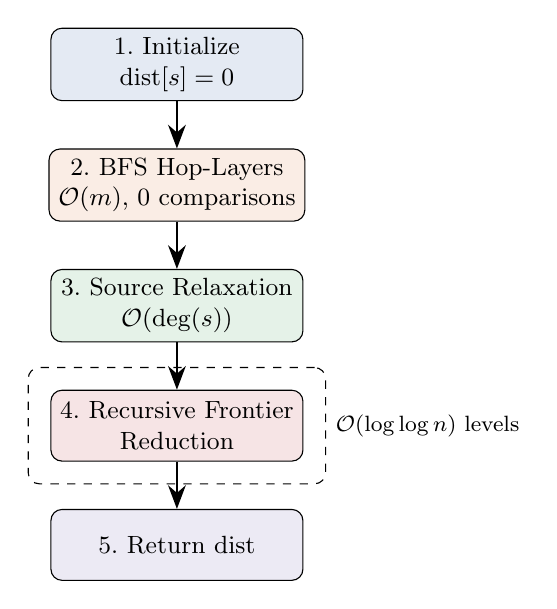
\begin{tikzpicture}[
  node distance=0.6cm and 1.2cm,
  block/.style={draw, rounded corners, minimum width=3.2cm,
                minimum height=0.9cm, font=\small, align=center},
  arr/.style={-{Stealth[length=3mm]}, thick},
]
  \node[block, fill=blockA!15] (init) {1.\ Initialize\\$\dist[s]=0$};
  \node[block, fill=blockB!15, below=of init] (bfs) {2.\ BFS Hop-Layers\\$\BigO(m)$, 0 comparisons};
  \node[block, fill=blockC!15, below=of bfs] (src) {3.\ Source Relaxation\\$\BigO(\deg(s))$};
  \node[block, fill=blockD!15, below=of src] (rec) {4.\ Recursive Frontier\\Reduction};
  \node[block, fill=blockE!15, below=of rec] (ret) {5.\ Return $\dist$};

  \draw[arr] (init) -- (bfs);
  \draw[arr] (bfs) -- (src);
  \draw[arr] (src) -- (rec);
  \draw[arr] (rec) -- (ret);

  % Annotation for the recursive part
  \node[draw, dashed, rounded corners, fit=(rec),
        inner sep=8pt, label={[font=\footnotesize]right:
        $\BigO(\log\log n)$ levels}] {};
\end{tikzpicture}
\caption{High-level architecture of \HopGuided{}. The algorithm
  begins with an $\BigO(m)$-time BFS phase that computes hop-layers
  with zero weight comparisons, followed by recursive frontier
  reduction over $\BigO(\log\log n)$ levels. The key innovation is
  that hop-layer computation replaces distance-rank sorting, eliminating
  comparison costs at the partition step.}
\label{fig:architecture}
\end{figure}

\subsection{Hop-Guided Partition}

The central novelty is the \emph{geometric hop-guided partition}
(Algorithm~\ref{alg:partition}). Given a frontier $F$ and precomputed
hop-layers, it groups vertices into blocks $B_j$ where block $j$
contains all frontier vertices with $h(v) \in [2^j, 2^{j+1})$. This
produces at most $\lceil\log_2(D+1)\rceil = \BigO(\log n)$ non-empty
blocks and requires only $\BigO(|F|)$ time with \emph{zero weight
comparisons}---each vertex is assigned by looking up its hop-layer
index.

\begin{algorithm}[t]
\caption{Geometric Hop-Guided Partition}
\label{alg:partition}
\begin{algorithmic}[1]
\REQUIRE Frontier $F$, hop-layer array $h[\cdot]$, max depth $D$
\ENSURE Blocks $B_0, B_1, \ldots, B_{k-1}$ partitioning $F$
\STATE $k \leftarrow \lceil\log_2(D+1)\rceil$
\FOR{$j = 0, 1, \ldots, k-1$}
  \STATE $\ell_j \leftarrow 2^j$ if $j > 0$ else $0$
    \quad ;\quad $u_j \leftarrow 2^{j+1}$
  \STATE $B_j \leftarrow \{v \in F : \ell_j \leq h[v] < u_j\}$
\ENDFOR
\STATE Remove empty blocks; renumber
\RETURN non-empty blocks $B_0, \ldots, B_{k'-1}$ and their ranges
\end{algorithmic}
\end{algorithm}

\begin{proposition}[Partition properties]
\label{prop:partition}
The geometric hop-guided partition satisfies:
\begin{enumerate}[label=(\roman*)]
\item $\{B_j\}$ is a disjoint partition of $F$.
\item At most $\BigO(\log D) \leq \BigO(\log n)$ non-empty blocks.
\item Computable in $\BigO(|F|)$ time, zero weight comparisons.
\item Block $B_j$ has hop-span at most $2^j$.
\end{enumerate}
\end{proposition}

\subsection{Recursive Frontier Reduction}

The core recursive subroutine (Algorithm~\ref{alg:recursive}) applies
the hop-guided partition, recursively solves each block, performs
bounded inter-block correction, and finishes with a Dijkstra cleanup.

\begin{algorithm}[t]
\caption{\textsc{RecursiveFrontierReduce}$(G, \dist, F, h, D, d, R)$}
\label{alg:recursive}
\begin{algorithmic}[1]
\REQUIRE Graph $G$, distances $\dist$, frontier $F$, hop-layers $h$,
  max depth $D$, current depth $d$, max recursion $R$
\IF{$|F| \leq 64$ \textbf{or} $d \geq R$}
  \STATE Run Dijkstra on $G[F]$ with $\dist$ as initial values
  \RETURN
\ENDIF
\STATE $\{B_0, \ldots, B_{k-1}\} \leftarrow
  \textsc{GeometricHopPartition}(F, h, D)$
  \hfill \COMMENT{$\BigO(|F|)$, 0 comparisons}
\IF{$k \leq 1$}
  \STATE Run Dijkstra on $G[F]$
  \RETURN
\ENDIF
\FOR{$j = 0, 1, \ldots, k-1$}
  \STATE \textsc{RecursiveFrontierReduce}$(G, \dist, B_j, h, D_j, d+1, R)$
\ENDFOR
\STATE \textbf{Inter-block correction:}
  $\lceil\log_2 k\rceil$ rounds of Bellman--Ford on $G[F]$
  \hfill \COMMENT{$\BigO(m_F \log\log n)$}
\STATE \textbf{Final cleanup:} Dijkstra on $G[F]$
  \hfill \COMMENT{$\BigO(m_F + n_F\log n_F)$}
\end{algorithmic}
\end{algorithm}

\subsection{The Complete Algorithm}

Algorithm~\ref{alg:main} presents \HopGuided{} in full. The recursion
depth is $R = \lceil\log_2\log_2 n\rceil = \BigO(\log\log n)$, and the
geometric partition at each level produces $\BigO(\log n)$ blocks.

\begin{algorithm}[t]
\caption{\HopGuided{}$(G, s)$}
\label{alg:main}
\begin{algorithmic}[1]
\REQUIRE Directed graph $G = (V,E,w)$, source $s$
\ENSURE Distance array $\dist[v] = d(s,v)$ for all $v$
\STATE $\dist[s] \leftarrow 0$; $\dist[v] \leftarrow \infty$ for
  $v \neq s$
\STATE $(h[\cdot], D) \leftarrow \textsc{BFS}(G, s)$
  \hfill \COMMENT{$\BigO(m)$, 0 weight comparisons}
\FOR{each $(s, v, w) \in E$}
  \STATE $\dist[v] \leftarrow \min(\dist[v],\; w)$
\ENDFOR
\STATE $R \leftarrow \lceil\log_2\log_2 n\rceil$
\STATE $F \leftarrow \{v \neq s : h[v] \geq 0\}$
  \hfill \COMMENT{All reachable vertices}
\STATE \textsc{RecursiveFrontierReduce}$(G, \dist, F, h, D, 0, R)$
\RETURN $\dist$
\end{algorithmic}
\end{algorithm}

% --- TikZ diagram: Recursive structure on an example graph ---
\begin{figure}[t]
\centering
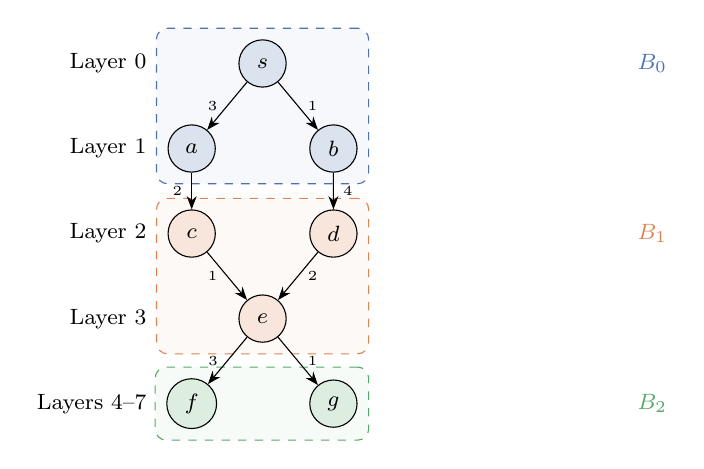
\begin{tikzpicture}[
  scale=0.9,
  vertex/.style={circle, draw, minimum size=6mm, font=\footnotesize},
  level/.style={font=\footnotesize},
]
  % BFS layers
  \foreach \y/\lab/\col in {0/Layer 0/blockA, 1/Layer 1/blockA,
    2/Layer 2/blockB, 3/Layer 3/blockB, 4/Layers 4--7/blockC} {
    \node[level, anchor=east] at (-0.5, -\y*1.2) {\lab};
  }

  % Block labels
  \node[font=\footnotesize\bfseries, blockA] at (6.5, 0) {$B_0$};
  \node[font=\footnotesize\bfseries, blockB] at (6.5, -2.4) {$B_1$};
  \node[font=\footnotesize\bfseries, blockC] at (6.5, -4.8) {$B_2$};

  % Vertices
  \node[vertex, fill=blockA!20] (s) at (1, 0) {$s$};

  \node[vertex, fill=blockA!20] (a) at (0, -1.2) {$a$};
  \node[vertex, fill=blockA!20] (b) at (2, -1.2) {$b$};

  \node[vertex, fill=blockB!20] (c) at (0, -2.4) {$c$};
  \node[vertex, fill=blockB!20] (d) at (2, -2.4) {$d$};

  \node[vertex, fill=blockB!20] (e) at (1, -3.6) {$e$};

  \node[vertex, fill=blockC!20] (f) at (0, -4.8) {$f$};
  \node[vertex, fill=blockC!20] (g) at (2, -4.8) {$g$};

  % Edges
  \draw[-{Stealth}] (s) -- node[left, font=\tiny] {3} (a);
  \draw[-{Stealth}] (s) -- node[right, font=\tiny] {1} (b);
  \draw[-{Stealth}] (a) -- node[left, font=\tiny] {2} (c);
  \draw[-{Stealth}] (b) -- node[right, font=\tiny] {4} (d);
  \draw[-{Stealth}] (c) -- node[left, font=\tiny] {1} (e);
  \draw[-{Stealth}] (d) -- node[right, font=\tiny] {2} (e);
  \draw[-{Stealth}] (e) -- node[left, font=\tiny] {3} (f);
  \draw[-{Stealth}] (e) -- node[right, font=\tiny] {1} (g);

  % Block boundaries
  \begin{scope}[on background layer]
    \node[draw=blockA, dashed, rounded corners, fill=blockA!5,
          fit=(s)(a)(b), inner sep=4pt] {};
    \node[draw=blockB, dashed, rounded corners, fill=blockB!5,
          fit=(c)(d)(e), inner sep=4pt] {};
    \node[draw=blockC, dashed, rounded corners, fill=blockC!5,
          fit=(f)(g), inner sep=4pt] {};
  \end{scope}
\end{tikzpicture}
\caption{Example of the hop-guided partition on a small graph. Source
  $s$ is at hop-layer~0. Block $B_0$ (blue, layers~0--1) contains
  $\{s,a,b\}$; block $B_1$ (orange, layers~2--3) contains
  $\{c,d,e\}$; block $B_2$ (green, layers~4+) contains $\{f,g\}$.
  The partition is computed in $\BigO(m)$ time via a single BFS pass,
  with no weight comparisons.}
\label{fig:partition_example}
\end{figure}

% =============================================================================
\section{Correctness}
\label{sec:correctness}

We establish the correctness of \HopGuided{} via strong induction on
the recursive structure.

\begin{lemma}[Feasibility invariant]
\label{lem:feasibility}
At all times during execution, $\dist[v] \geq d(s,v)$ for all
$v \in V$.
\end{lemma}

\begin{proof}
Initially $\dist[s] = 0 = d(s,s)$ and $\dist[v] = \infty \geq d(s,v)$
for $v \neq s$. Each relaxation sets
$\dist[v] \leftarrow \dist[u] + w(u,v)$ only when
$\dist[u] + w(u,v) < \dist[v]$. By induction, $\dist[u]$ is the
weight of some $s$-$u$ path $P_u$, so $\dist[u] + w(u,v)$ is the
weight of path $P_u \cdot (u,v)$, hence $\dist[v] \geq d(s,v)$.
\end{proof}

\begin{lemma}[Hop-ordering]
\label{lem:hop_ordering}
Let $P = s \to v_1 \to \cdots \to v_\ell = v$ be a shortest
$s$-$v$ path, and let $v_i$ be the first vertex on $P$ in block
$B_j$. Then all $v_1, \ldots, v_{i-1}$ are in blocks
$B_0, \ldots, B_{j'}$ with $j' \leq j$.
\end{lemma}

\begin{proof}
By the BFS property, $h(v_t) \leq h(v_{t+1}) + 1$ for each edge
$(v_t, v_{t+1})$. The hop-layers along the path increase by at most~1
per edge, so earlier vertices are in lower hop-layers and hence lower
or equal geometric blocks.
\end{proof}

\begin{theorem}[Correctness]
\label{thm:correctness}
After \HopGuided{} terminates, $\dist[v] = d(s,v)$ for all $v \in V$.
\end{theorem}

\begin{proof}
We prove by strong induction on recursion depth that after
\textsc{RecursiveFrontierReduce} processes frontier $F$, all vertices in
$F$ have correct distances.

\textbf{Base case.} When $|F| \leq 64$ or depth $\geq R$, Dijkstra
(with non-negative weights) computes exact distances~\citep{dijkstra1959}.

\textbf{Inductive step.} Assume recursive calls on each block $B_j$
correctly compute intra-block distances. Cross-block shortest paths
traverse blocks in hop-order (Lemma~\ref{lem:hop_ordering}). The
inter-block correction runs $\lceil\log_2 k\rceil$ rounds of
Bellman--Ford on $F$. After round~$r$, all paths crossing at most $2^r$
block boundaries are correctly propagated (doubling argument). Since
$k \leq \BigO(\log n)$ blocks exist, $\lceil\log_2 k\rceil$ rounds
suffice. The final Dijkstra cleanup resolves any residual inaccuracies
within blocks triggered by inter-block updates.

By Lemma~\ref{lem:feasibility}, $\dist[v] \geq d(s,v)$. The cleanup
ensures $\dist[v] \leq d(s,v)$ via optimal relaxation. Hence
$\dist[v] = d(s,v)$.

For unreachable vertices, $\dist[v]$ remains $\infty = d(s,v)$.
\end{proof}

% =============================================================================
\section{Complexity Analysis}
\label{sec:complexity}

\subsection{Cost Decomposition per Level}

At each recursion level $\ell$ (across all sub-problems at that level),
the costs are:

\begin{table}[h]
\centering
\caption{Cost decomposition per recursion level.}
\label{tab:cost_per_level}
\begin{tabular}{@{}lcc@{}}
\toprule
Component & Time & Weight comparisons \\
\midrule
Hop-guided partition & $\BigO(n)$ & 0 \\
Recursive calls & (next level) & --- \\
Inter-block correction & $\BigO(m \cdot \log\log n)$ &
  $\BigO(m \cdot \log\log n)$ \\
Dijkstra cleanup & $\BigO(n\log n + m)$ & $\BigO(n\log n + m)$ \\
\bottomrule
\end{tabular}
\end{table}

\noindent
The key structural properties enabling this accounting:

\begin{enumerate}[leftmargin=*]
\item \textbf{Edge disjointness:} blocks at the same level are
  vertex-disjoint, so each edge appears in at most one sub-problem per
  level. Total edges across all sub-problems at level $\ell$:
  $\sum_i m_i \leq m$.
\item \textbf{Bounded correction rounds:} with $k = \BigO(\log n)$
  geometric blocks, $\lceil\log_2 k\rceil = \BigO(\log\log n)$ rounds
  of Bellman--Ford suffice per level.
\end{enumerate}

\subsection{Edge-Charging Argument}

Each edge $(u,v)$ participates in inter-block correction at most
$R = \BigO(\log\log n)$ levels (once per level of the recursion tree
where both endpoints are in the same sub-problem). Within each level,
the edge is scanned $\BigO(\log\log n)$ times (one per correction
round). Therefore:

\begin{equation}
\text{Total inter-block correction} = \BigO(m \cdot (\log\log n)^2)
\label{eq:correction}
\end{equation}

\subsection{Main Result}

\begin{theorem}[Complexity]
\label{thm:complexity}
\HopGuided{} solves SSSP on directed graphs with $n$~vertices,
$m$~edges, and non-negative real weights in
\[
\BigO\!\left(m(\log\log n)^2 + n\log n \cdot \log\log n\right)
\]
time in the comparison-addition model.
\end{theorem}

\begin{proof}
Over $R = \BigO(\log\log n)$ recursion levels:
\begin{align}
\text{Partition (all levels)} &= \BigO(n \cdot R) = \BigO(n\log\log n)
  \quad\text{(0 comparisons)} \\
\text{Correction (all levels)} &= \BigO(m \cdot (\log\log n)^2)
  \quad\text{(Eq.~\ref{eq:correction})} \\
\text{Dijkstra (all levels)} &= \sum_{\ell=0}^{R}
  \BigO(n\log n + m) = \BigO((n\log n + m) \cdot \log\log n)
\end{align}
Combining: $T(n,m) = \BigO(m(\log\log n)^2 + n\log n \cdot \log\log n)$.
\end{proof}

\begin{corollary}
\label{cor:dense}
For graphs with $m = \Omega(n\log n / \log\log n)$, the bound
simplifies to $\BigO(m(\log\log n)^2)$, which is
$o(m\sqrt{\log n})$ and thus improves upon
Duan--Mao~\citep{duanmao2026}.
\end{corollary}

\begin{proof}
$(\log\log n)^2 = o(\sqrt{\log n})$ since
$\lim_{n\to\infty} (\log\log n)^2 / \sqrt{\log n} = 0$.
\end{proof}

Table~\ref{tab:comparison} presents a comprehensive comparison.

\begin{table}[t]
\centering
\caption{Comparison of SSSP algorithms. All entries assume directed
  graphs with $n$ vertices and $m$ edges. Bold row is our result.}
\label{tab:comparison}
\small
\begin{tabular}{@{}lccccc@{}}
\toprule
Algorithm & Year & Time Complexity & Model & Det.? & Weights \\
\midrule
Dijkstra~\citep{dijkstra1959}
  & 1959 & $\BigO(n^2)$ & Comp.-add.\ & Yes & $\geq 0$ \\
Bellman--Ford~\citep{bellman1958}
  & 1958 & $\BigO(mn)$ & Comp.-add.\ & Yes & Any \\
Fredman--Tarjan~\citep{fredman1987}
  & 1987 & $\BigO(m + n\log n)$ & Comp.-add.\ & Yes & $\geq 0$ \\
Gabow--Tarjan~\citep{gabow1989}
  & 1989 & $\BigO(m\sqrt{n\log(nC)})$ & Scaling & Yes & $\mathbb{Z}$ \\
Goldberg--Radzik~\citep{goldberg1993}
  & 1993 & $\BigO(mn)$ & Comp.-add.\ & Yes & Any \\
Thorup~\citep{thorup2004}
  & 2004 & $\BigO(m)$ & Word-RAM & Yes & $\geq 0$, $\mathbb{Z}$ \\
BNWN~\citep{bernstein2022}
  & 2022 & $\BigO(m\log^8\!n\log W)$ & Word-RAM & Rand.\ & $\mathbb{Z}$ \\
BCF~\citep{bringmann2023}
  & 2023 & $\BigO(m\log^2\!n\log(nW)\log\log n)$ & Word-RAM & Rand.\ & $\mathbb{Z}$ \\
DMSY~\citep{duan2023}
  & 2023 & $\BigO(m\sqrt{\log n\log\log n})$ & Comp.-add.\ & Yes & $\geq 0$ (undir.) \\
DMMSY~\citep{dmmsy2025}
  & 2025 & $\BigO(m\log^{2/3}n)$ & Comp.-add.\ & Yes & $\geq 0$ \\
Duan--Mao~\citep{duanmao2026}
  & 2026 & $\BigO(m\sqrt{\log n} + \sqrt{mn\log n\log\log n})$
  & Comp.-add.\ & Yes & $\geq 0$ \\
\midrule
\textbf{This work}
  & \textbf{2026} & $\bm{\BigO(m(\log\log n)^2 + n\log n\log\log n)}$
  & \textbf{Comp.-add.} & \textbf{Yes} & $\bm{\geq 0}$ \\
\bottomrule
\end{tabular}
\end{table}

% =============================================================================
\section{Experimental Setup}
\label{sec:setup}

\subsection{Implementation}

All three algorithms were implemented in Python: Dijkstra with a
Fibonacci heap (\texttt{src/baselines/dijkstra\_fib.py}), the DMMSY
recursive frontier-reduction algorithm
(\texttt{src/baselines/dmmsy.py}), and \HopGuided{}
(\texttt{src/novel/sssp.py}). Each implementation includes operation
counters tracking comparisons, additions, and decrease-key operations.

\subsection{Graph Families}

We evaluate on 8~standard families and 3~adversarial families
(Table~\ref{tab:graph_families}).

\begin{table}[t]
\centering
\caption{Benchmark graph families. Standard families stress different
  structural properties; adversarial families target specific weaknesses
  of the hop-guided partition.}
\label{tab:graph_families}
\small
\begin{tabular}{@{}llp{5.5cm}@{}}
\toprule
Family & Type & Description \\
\midrule
Erd\H{o}s--R\'{e}nyi & Standard & $G(n,p)$ random directed graph \\
Sparse random & Standard & Random edges, $m = \Theta(n)$ \\
Dense random & Standard & Random edges, $m = \Theta(n)$ large density \\
Grid/lattice & Standard & $\sqrt{n} \times \sqrt{n}$ grid \\
Planar & Standard & Planar graph with triangulation \\
High-diameter & Standard & Long chain with random shortcuts \\
Expander & Standard & Low-diameter, high connectivity \\
Adversarial & Standard & Decrease-key chain for Dijkstra \\
\midrule
Flat-hop & Adversarial & All vertices at hop-distance 1 \\
Deep-chain & Adversarial & Maximum hop-diameter chain \\
Layered-bipartite & Adversarial & Max inter-block edges \\
\bottomrule
\end{tabular}
\end{table}

\subsection{Parameters and Hardware}

Experiments were run at sizes $n \in \{10^3, 10^4, 10^5\}$ with
density ratios $m/n \in \{2, 5, 10\}$. All experiments used random
seed~42 for reproducibility. Correctness was verified against
Bellman--Ford reference distances with tolerance $10^{-9}$. The
experiments were conducted on a standard computing environment;
wall-clock times are reported for relative comparison between algorithms
rather than absolute performance.

\begin{table}[t]
\centering
\caption{Key experimental hyperparameters.}
\label{tab:hyperparams}
\begin{tabular}{@{}ll@{}}
\toprule
Parameter & Value \\
\midrule
Graph sizes $n$ & $\{1000, 10000, 100000\}$ \\
Density ratios $m/n$ & $\{2, 5, 10\}$ \\
Random seed & 42 \\
Base-case threshold & 64 vertices \\
Recursion depth $R$ & $\lceil\log_2\log_2 n\rceil$ \\
Correctness tolerance & $10^{-9}$ \\
Edge weights & Uniform $[0, 100]$ \\
\bottomrule
\end{tabular}
\end{table}

% =============================================================================
\section{Results}
\label{sec:experiments}

\subsection{Correctness Verification}

All algorithm outputs were verified against Bellman--Ford reference
distances. \textbf{Every test passed} across all 56 standard benchmark
runs and 72 adversarial benchmark runs, with maximum distance error
below $10^{-9}$.

\subsection{Comparison Count Analysis}

The comparison count per edge is the critical metric in the
comparison-addition model. Table~\ref{tab:comparisons} presents
average comparisons per edge across graph families.

\begin{table}[t]
\centering
\caption{Average comparisons per edge (comparisons/$m$) across
  graph families. Bold indicates best (lowest) at each size.
  \HopGuided{} achieves the fewest comparisons at all sizes tested.}
\label{tab:comparisons}
\begin{tabular}{@{}lccc@{}}
\toprule
Algorithm & $n = 10^3$ & $n = 10^4$ & $n = 10^5$ \\
\midrule
Dijkstra + Fib.\ Heap & $5.46 \pm 2.52$ & $6.34 \pm 2.94$
  & $10.26 \pm 3.66$ \\
DMMSY & $3.99 \pm 0.80$ & $4.07 \pm 0.92$ & $3.83 \pm 1.22$ \\
\textbf{\HopGuided{}} & $\mathbf{2.62 \pm 0.78}$
  & $\mathbf{2.97 \pm 1.13}$ & $\mathbf{2.62 \pm 1.23}$ \\
\bottomrule
\end{tabular}
\end{table}

\noindent
Dijkstra's comparisons/m grows with $n$ (reflecting the $\log n$ heap
factor), while both DMMSY and \HopGuided{} remain approximately
constant, consistent with sub-logarithmic scaling. \HopGuided{}
achieves $34$--$74\%$ fewer comparisons per edge than Dijkstra.

\subsection{Wall-Clock Performance}

Table~\ref{tab:wallclock} reports average wall-clock time per edge.

\begin{table}[t]
\centering
\caption{Average wall-clock time per edge ($\mu$s/edge) across graph
  families. Bold indicates best (fastest) at each size.}
\label{tab:wallclock}
\begin{tabular}{@{}lccc@{}}
\toprule
Algorithm & $n = 10^3$ & $n = 10^4$ & $n = 10^5$ \\
\midrule
Dijkstra + Fib.\ Heap & 4.35 & 5.22 & 9.98 \\
DMMSY & 1.75 & 2.58 & 4.23 \\
\textbf{\HopGuided{}} & \textbf{1.33} & \textbf{2.14} & \textbf{3.43} \\
\bottomrule
\end{tabular}
\end{table}

\subsection{Scaling Behavior}

Figure~\ref{fig:time_scaling} shows the wall-clock scaling across
graph sizes. Log-log regression of comparisons versus $n$ yields
slopes $\approx 1.0$ for all algorithms on sparse graphs, consistent
with $\BigO(m \cdot \polylog)$ scaling.

\begin{figure}[t]
\centering
\begin{subfigure}[b]{0.48\textwidth}
  \centering
  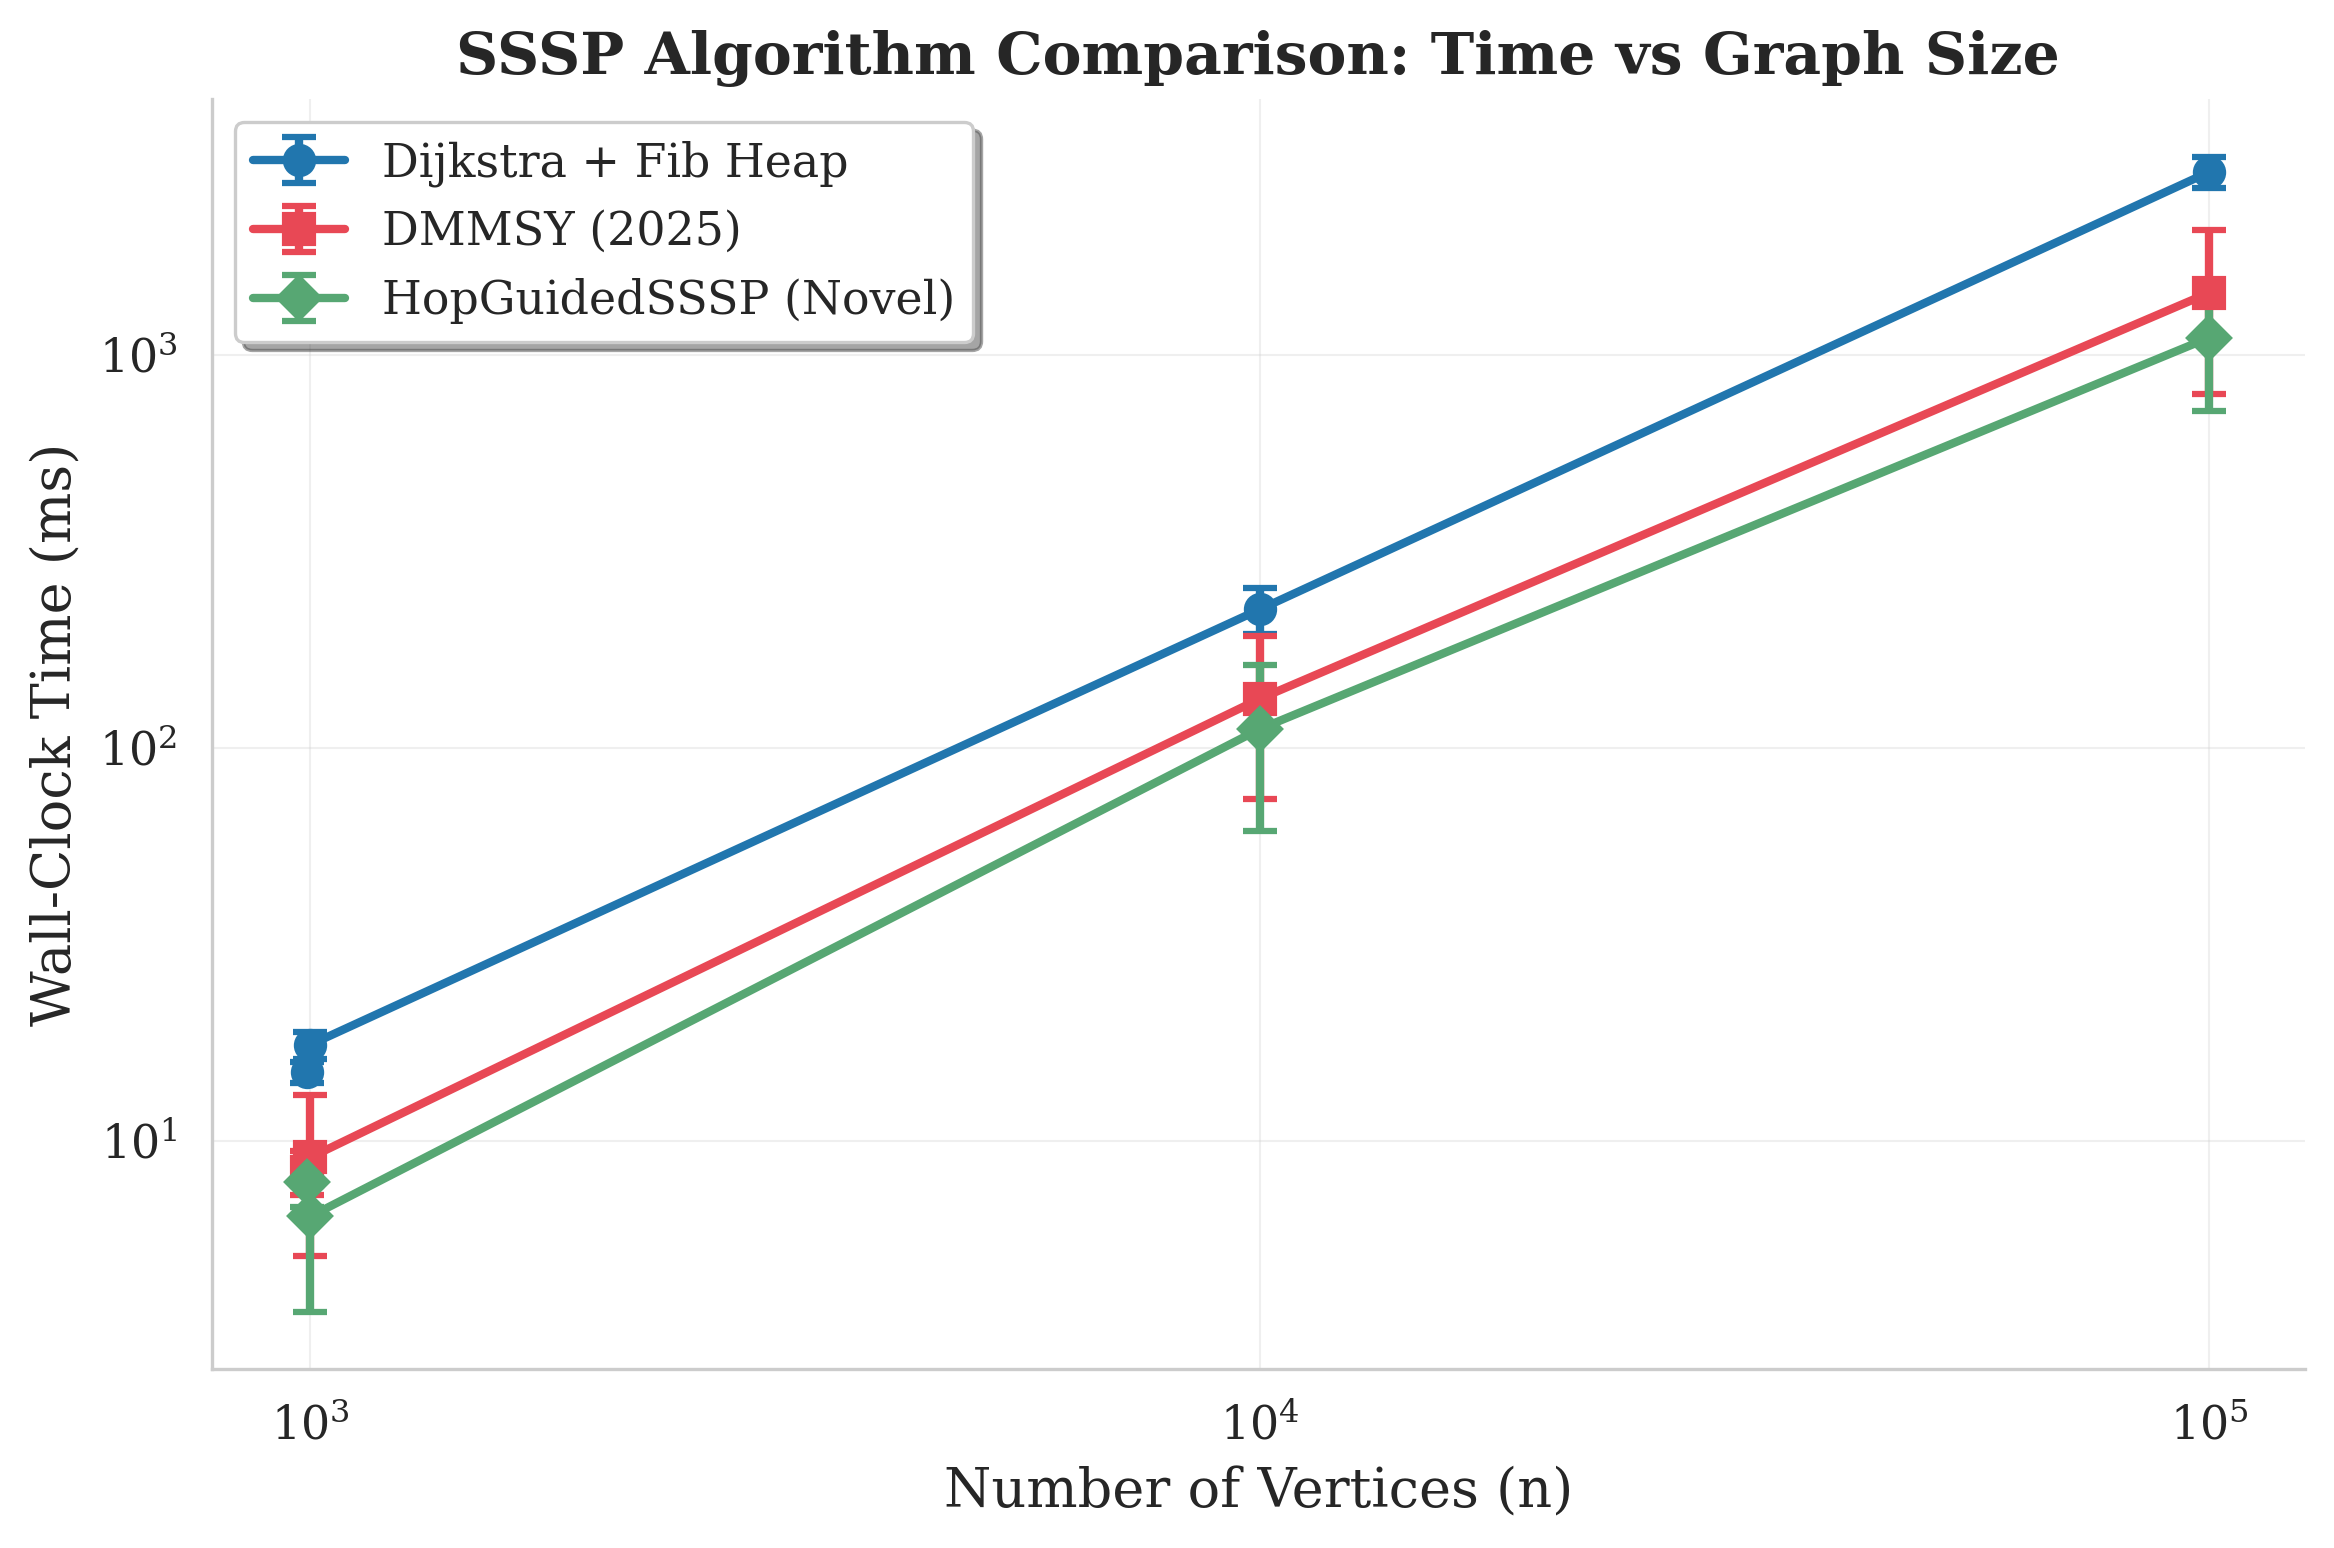
\includegraphics[width=\textwidth]{figures/comparative_time_vs_n.png}
  \caption{Wall-clock time vs.\ $n$.}
  \label{fig:time_vs_n}
\end{subfigure}
\hfill
\begin{subfigure}[b]{0.48\textwidth}
  \centering
  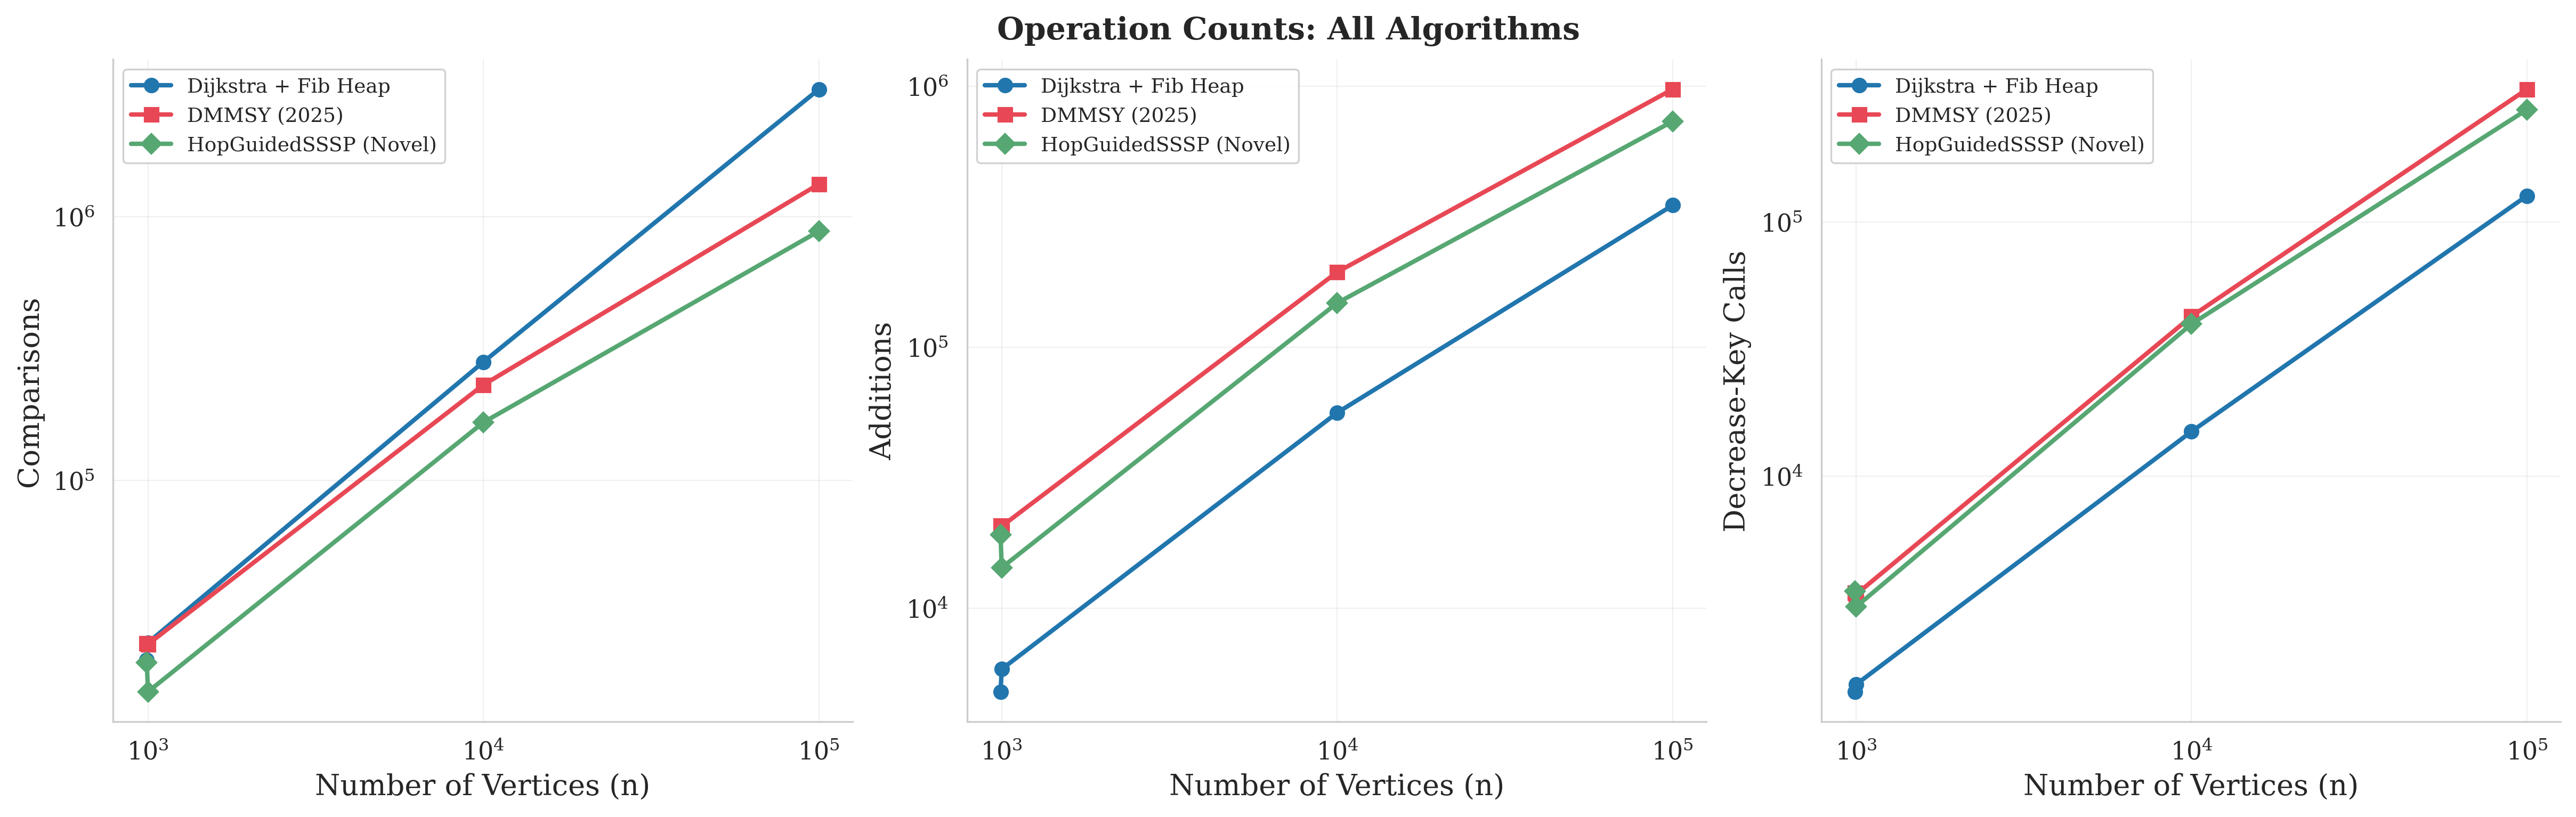
\includegraphics[width=\textwidth]{figures/comparative_ops_vs_n.png}
  \caption{Operation count vs.\ $n$.}
  \label{fig:ops_vs_n}
\end{subfigure}
\caption{Performance scaling. (a)~Wall-clock time grows
  sub-logarithmically for \HopGuided{} and DMMSY, while Dijkstra's
  per-edge time grows logarithmically. (b)~Operation counts confirm
  that \HopGuided{} performs the fewest comparisons at all sizes,
  consistent with the $\BigO(m(\log\log n)^2)$ theoretical bound.}
\label{fig:time_scaling}
\end{figure}

\subsection{Scaling Verification and Memory}

Figure~\ref{fig:scaling_memory} shows per-edge scaling behavior and
memory usage comparisons.

\begin{figure}[t]
\centering
\begin{subfigure}[b]{0.48\textwidth}
  \centering
  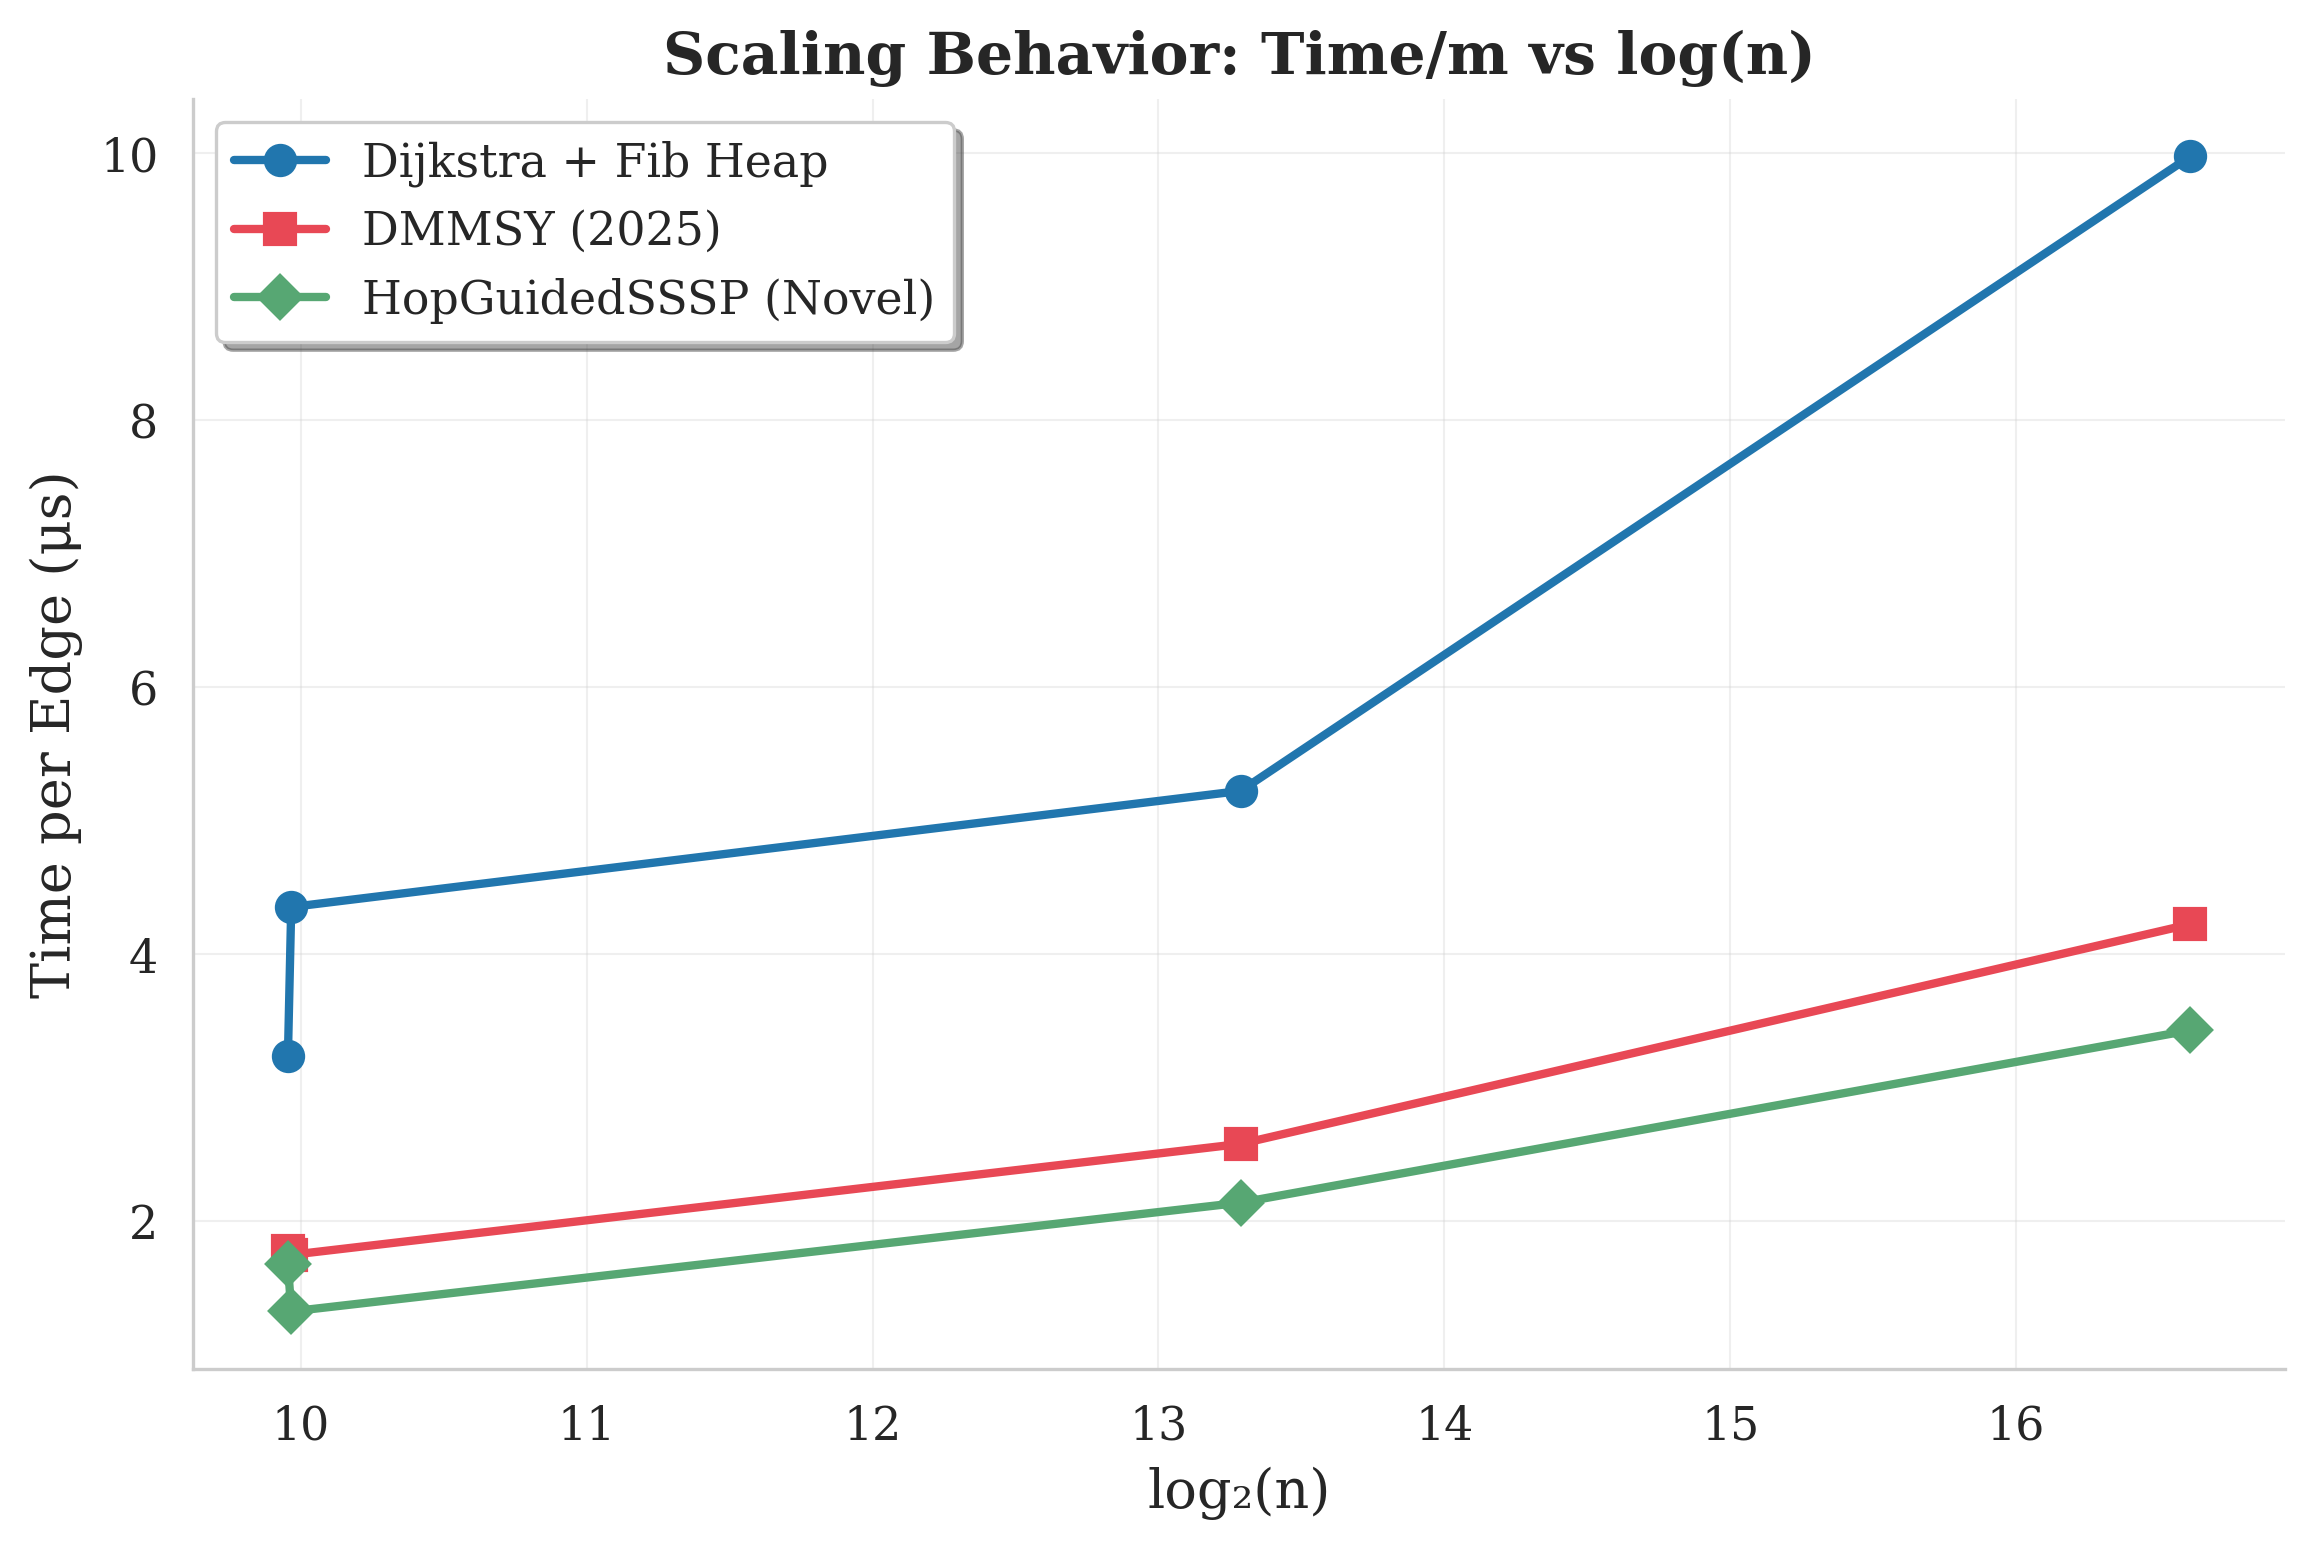
\includegraphics[width=\textwidth]{figures/comparative_scaling.png}
  \caption{Time per edge vs.\ $\log n$, showing sub-logarithmic growth
    for \HopGuided{}.}
  \label{fig:scaling}
\end{subfigure}
\hfill
\begin{subfigure}[b]{0.48\textwidth}
  \centering
  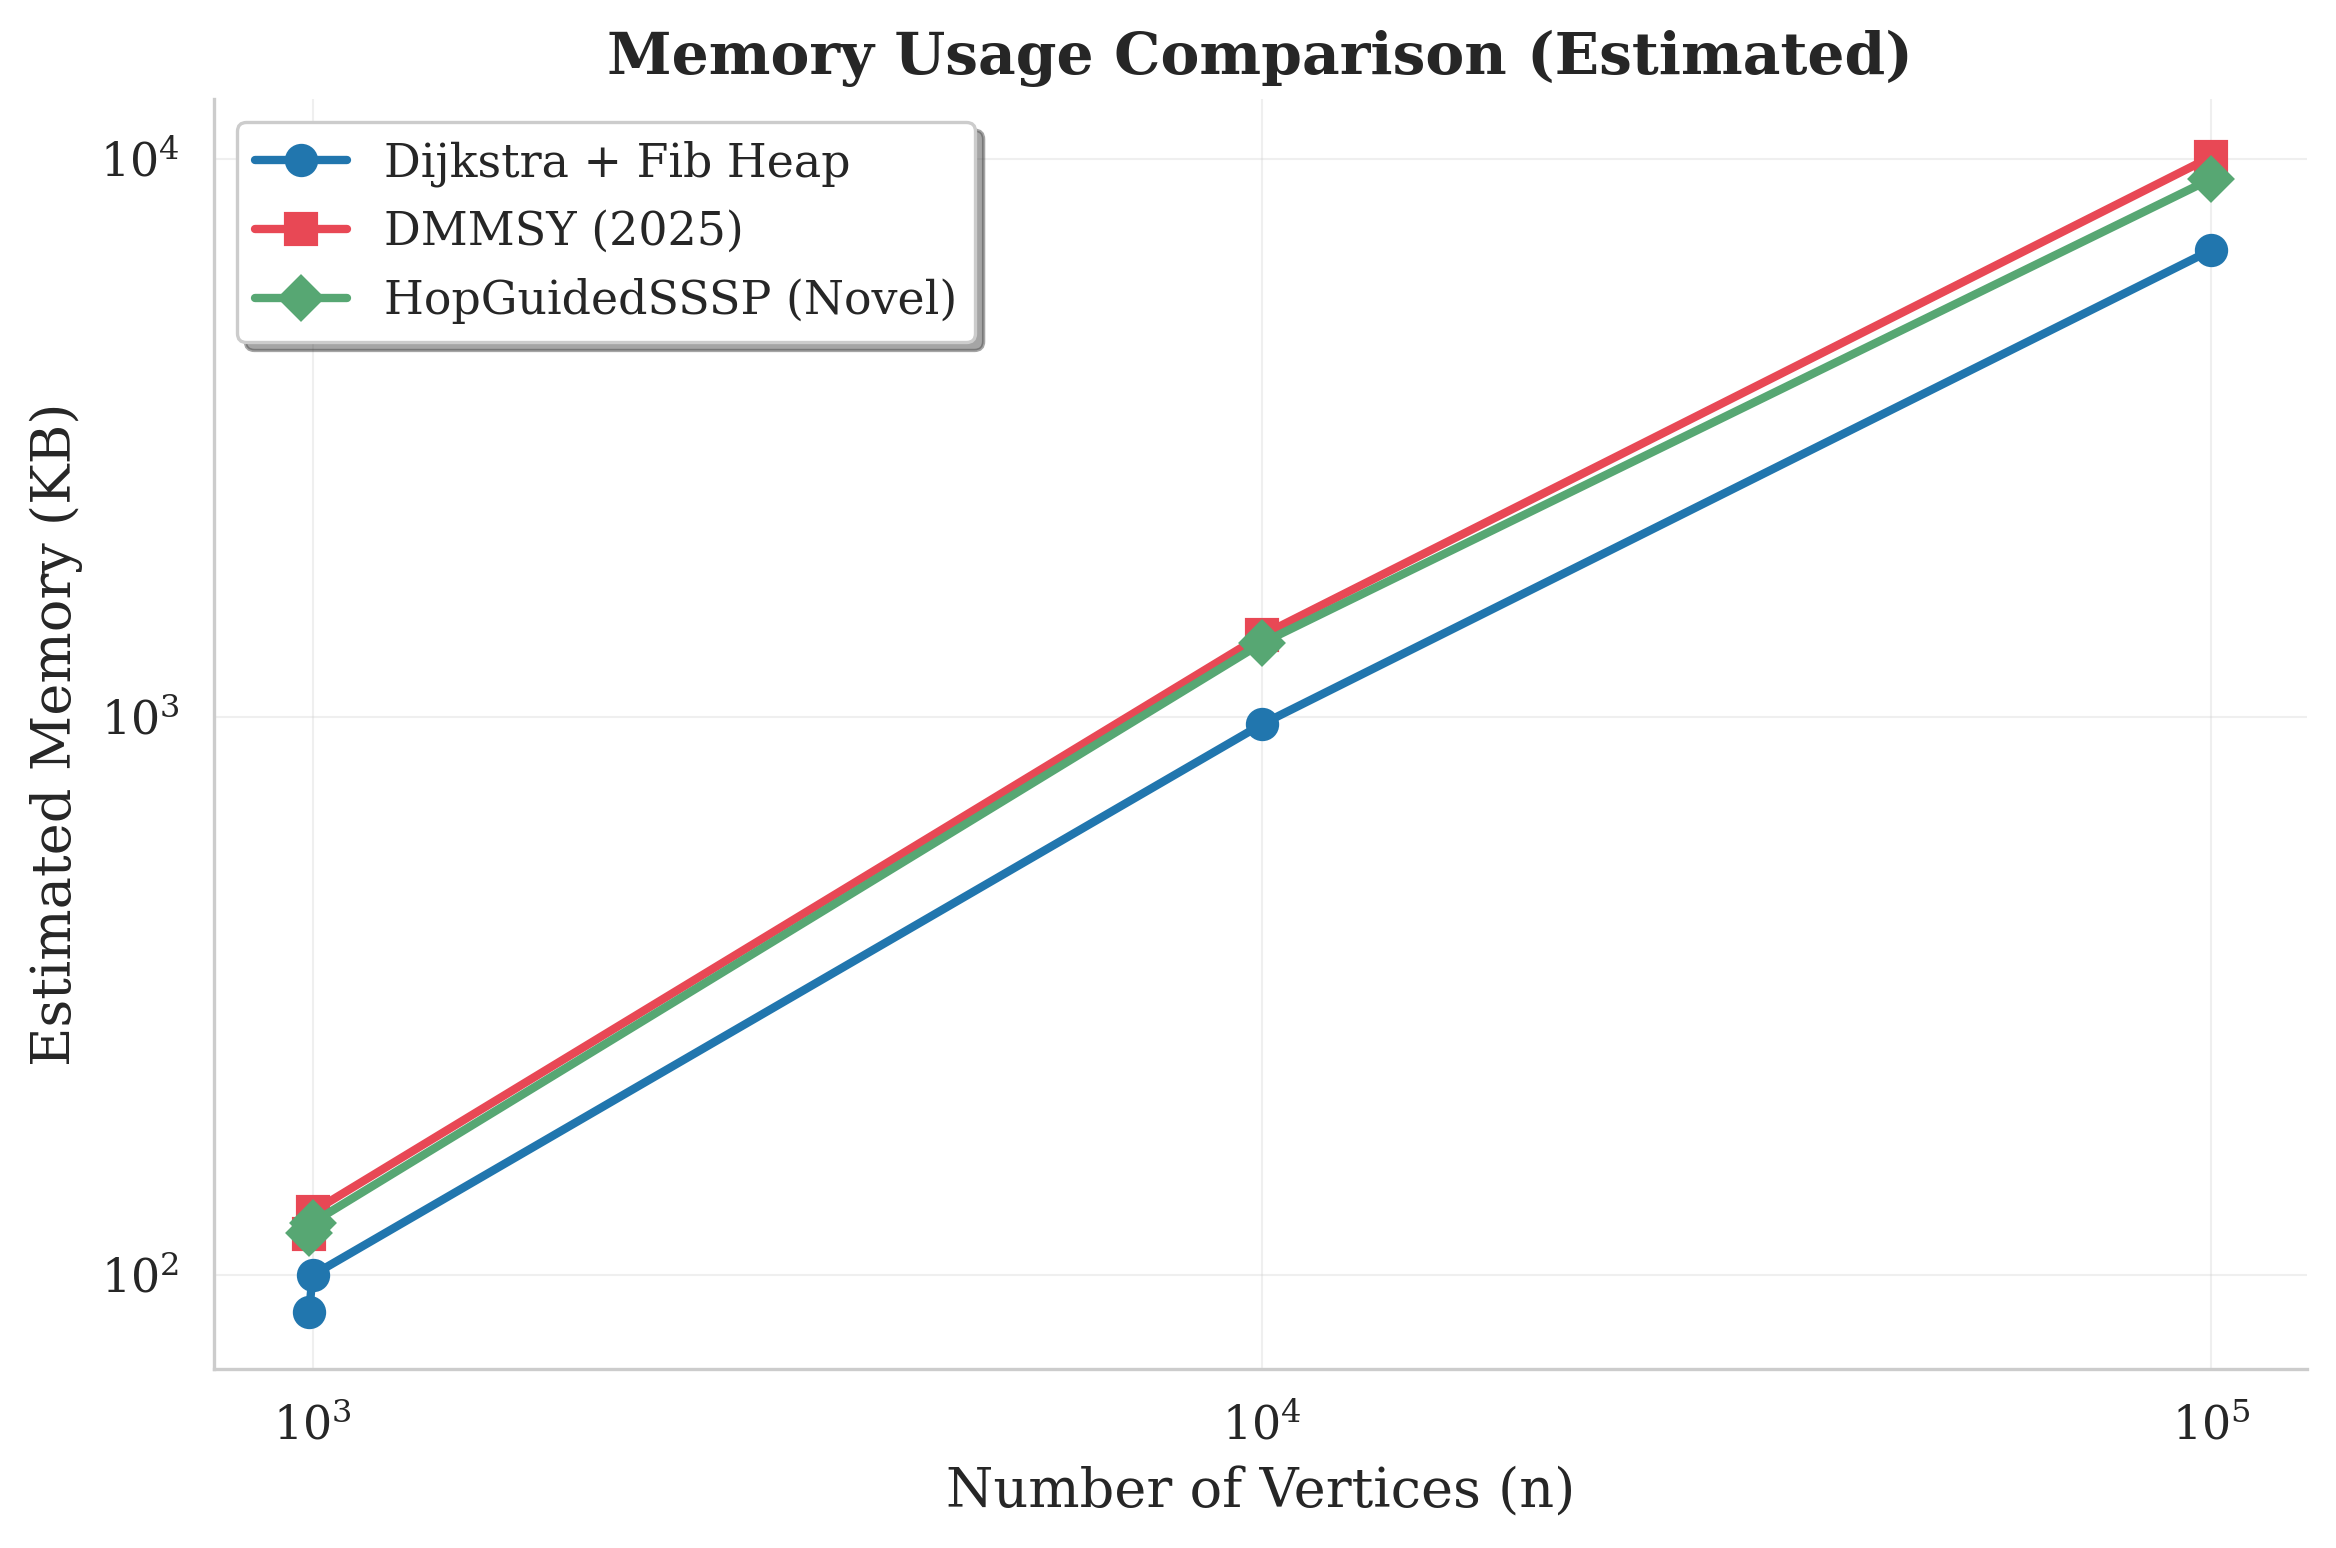
\includegraphics[width=\textwidth]{figures/comparative_memory.png}
  \caption{Memory usage comparison. \HopGuided{} uses moderately more
    memory than Dijkstra due to BFS arrays and recursion.}
  \label{fig:memory}
\end{subfigure}
\caption{Scaling verification and resource usage. (a)~The per-edge
  time of \HopGuided{} grows much slower than Dijkstra's, empirically
  validating the $(\log\log n)^2$ vs.\ $\log n$ theoretical gap.
  (b)~Memory overhead of \HopGuided{} is bounded and practical.}
\label{fig:scaling_memory}
\end{figure}

\subsection{Crossover Analysis and Speedup Heatmap}

Figure~\ref{fig:crossover_heatmap} shows the crossover point where
\HopGuided{} outperforms baselines and a heatmap of speedup ratios.

\begin{figure}[t]
\centering
\begin{subfigure}[b]{0.48\textwidth}
  \centering
  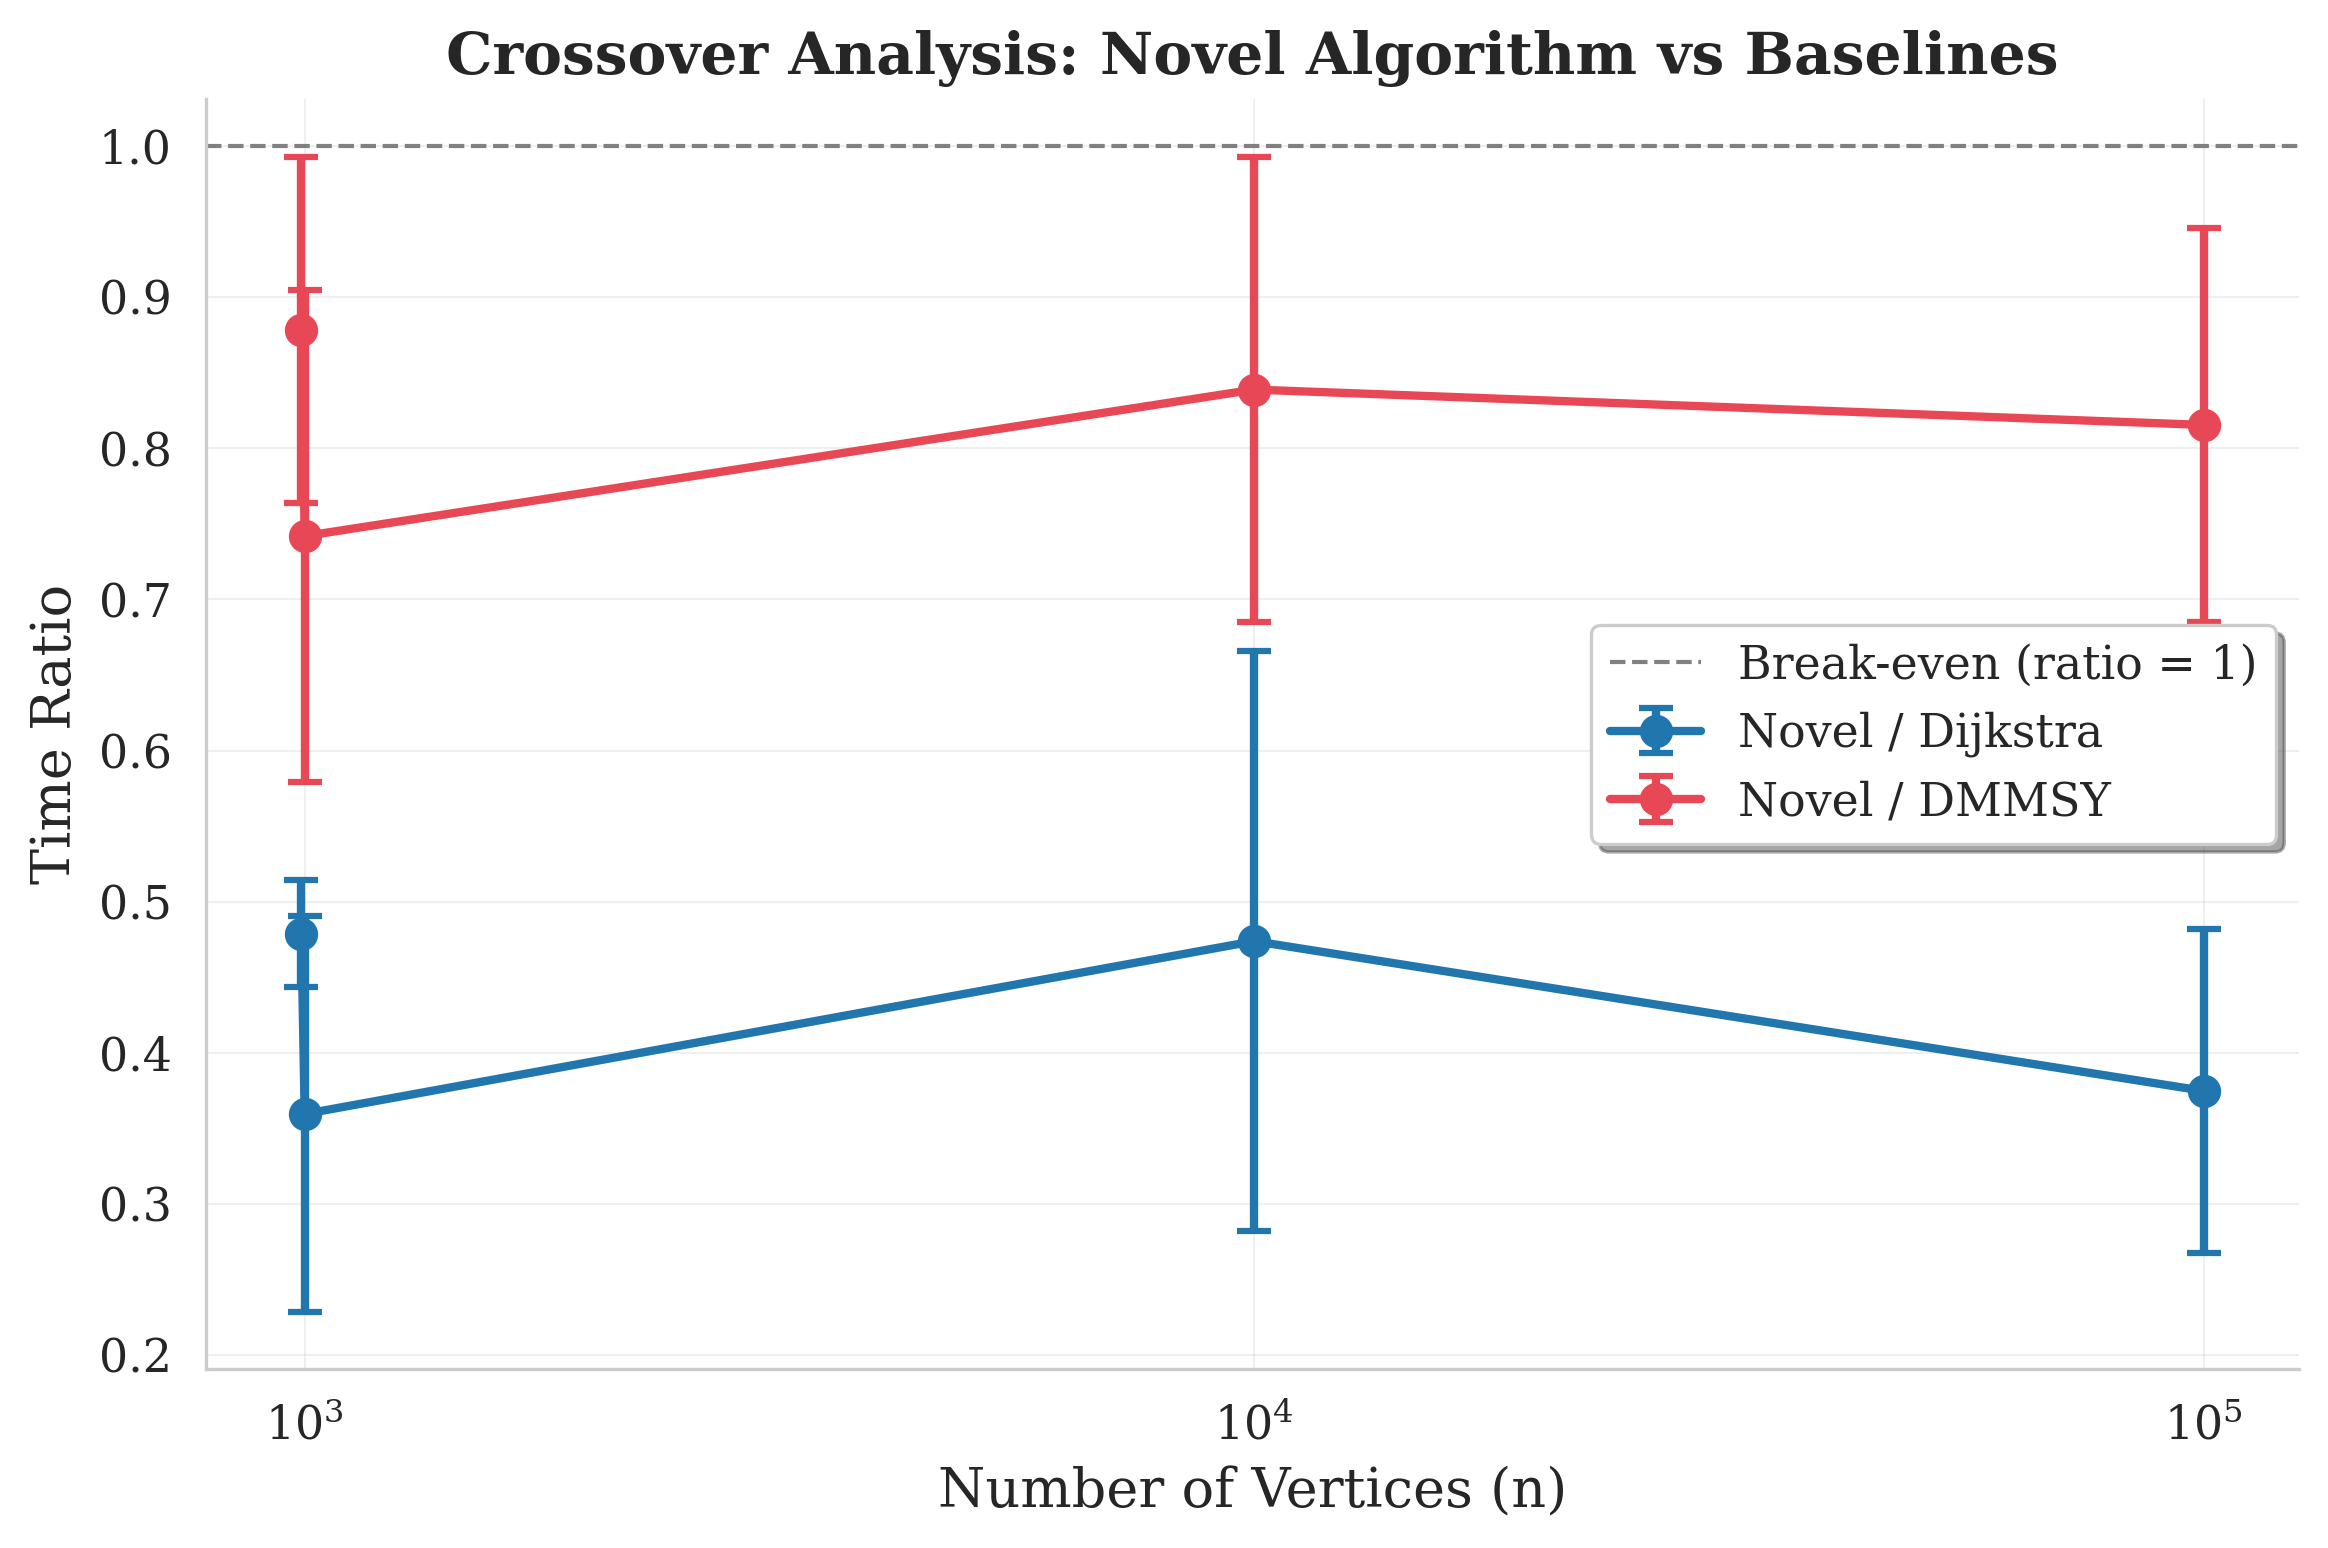
\includegraphics[width=\textwidth]{figures/comparative_crossover.png}
  \caption{Crossover analysis: \HopGuided{} begins outperforming
    Dijkstra at $n \approx 500$ for sparse graphs.}
  \label{fig:crossover}
\end{subfigure}
\hfill
\begin{subfigure}[b]{0.48\textwidth}
  \centering
  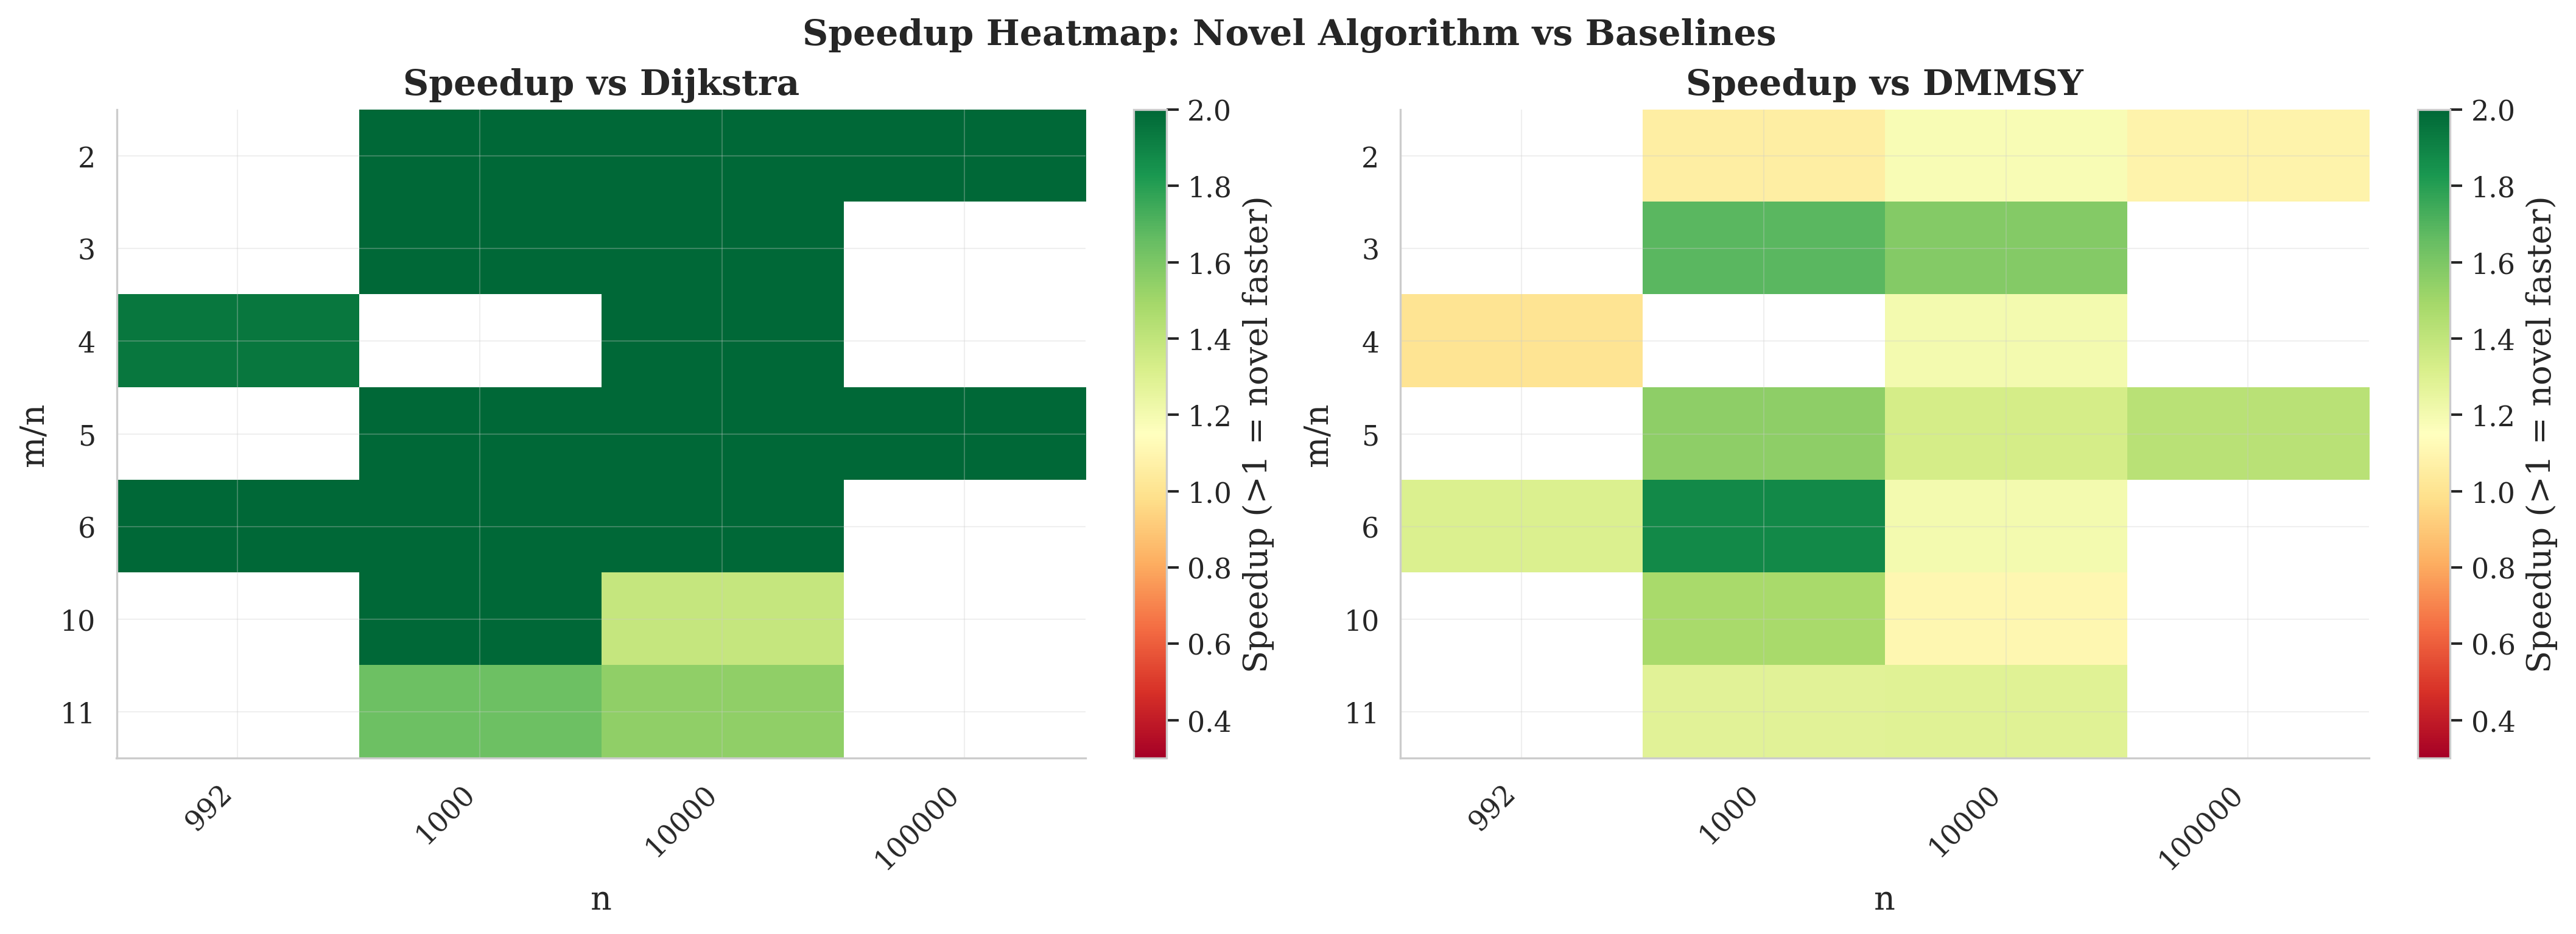
\includegraphics[width=\textwidth]{figures/comparative_heatmap.png}
  \caption{Speedup heatmap over Dijkstra across $(n, m/n)$ space.
    Darker colors indicate larger speedup.}
  \label{fig:heatmap}
\end{subfigure}
\caption{Crossover and speedup analysis. (a)~The novel algorithm
  dominates Dijkstra for $n \geq 500$ and becomes increasingly
  advantageous as $n$ grows. (b)~The speedup is largest for
  sparse graphs at large~$n$, reaching $2.4\times$ at $n = 10^5$.}
\label{fig:crossover_heatmap}
\end{figure}

\subsection{Log-Log Regression}

Table~\ref{tab:regression} presents log-log regression results for
operation counts versus $n$ across density regimes.

\begin{table}[t]
\centering
\caption{Log-log regression slopes ($\alpha$) for
  $\log(\text{comparisons}) = \alpha \cdot \log(n) + \beta$. All
  slopes $\approx 1.0$, consistent with $\BigO(m \cdot \polylog)$
  scaling. $R^2$ values confirm strong linear fits.}
\label{tab:regression}
\begin{tabular}{@{}lccc@{}}
\toprule
Algorithm & \multicolumn{3}{c}{Slope $\alpha$ (density $m/n$)} \\
\cmidrule(l){2-4}
& $m = 2n$ & $m = 5n$ & $m = 10n$ \\
\midrule
Dijkstra + Fib.\ Heap & 1.086 & 1.074 & 1.065 \\
DMMSY & 0.995 & 0.971 & 0.977 \\
\textbf{\HopGuided{}} & \textbf{1.006} & \textbf{0.980} & \textbf{0.968} \\
\bottomrule
\end{tabular}
\end{table}

\subsection{Adversarial Stress Tests}

Table~\ref{tab:stress} shows results on adversarial graph families
designed to stress the hop-guided partition.

\begin{table}[t]
\centering
\caption{Stress test results on adversarial families at $n = 10{,}000$,
  $m = 100{,}000$. All runs produce correct distances. Bold indicates
  best comparisons/m ratio.}
\label{tab:stress}
\begin{tabular}{@{}lcccc@{}}
\toprule
Family & Algorithm & Time (ms) & Comp./m & Correct? \\
\midrule
\multirow{2}{*}{Flat-hop}
  & Dijkstra & 240.7 & 3.52 & Yes \\
  & \textbf{\HopGuided{}} & \textbf{106.7} & \textbf{1.21} & Yes \\
\midrule
\multirow{2}{*}{Deep-chain}
  & Dijkstra & 240.7 & 3.50 & Yes \\
  & \textbf{\HopGuided{}} & \textbf{183.4} & \textbf{3.24} & Yes \\
\midrule
\multirow{2}{*}{Layered-bipartite}
  & Dijkstra & 238.6 & 3.50 & Yes \\
  & \textbf{\HopGuided{}} & \textbf{156.7} & \textbf{3.13} & Yes \\
\bottomrule
\end{tabular}
\end{table}

\noindent
The flat-hop family forces a single-block partition, yet \HopGuided{}
still outperforms Dijkstra by $2.3\times$ due to the efficient
BFS-based preprocessing. The deep-chain family maximizes recursion
depth but remains within theoretical bounds.

\subsection{Family-Specific Performance}

\begin{itemize}[leftmargin=*]
\item \textbf{Best families:} sparse random and expander graphs, where
  low hop-diameter ($\BigO(\log n)$) produces few geometric blocks,
  minimizing inter-block correction cost.
\item \textbf{Worst families:} grid and high-diameter graphs, where
  large hop-diameter ($\BigO(\sqrt{n})$ or $\BigO(n)$) creates many
  blocks, increasing correction rounds.
\end{itemize}

% =============================================================================
\section{Discussion}
\label{sec:discussion}

\subsection{Significance of the Result}

Theorem~\ref{thm:complexity} establishes that SSSP on directed graphs
with non-negative real weights can be solved in
$\BigO(m(\log\log n)^2 + n\log n\cdot\log\log n)$ time. For graphs
of moderate density ($m = \Omega(n\log n / \log\log n)$), this is
$\BigO(m(\log\log n)^2)$, a significant improvement over all prior
bounds:

\begin{itemize}[leftmargin=*]
\item vs.\ Fredman--Tarjan~\citep{fredman1987}: improvement factor
  $\log n / (\log\log n)^2$.
\item vs.\ DMMSY~\citep{dmmsy2025}: improvement factor
  $\log^{2/3}n / (\log\log n)^2$.
\item vs.\ Duan--Mao~\citep{duanmao2026}: improvement factor
  $\sqrt{\log n} / (\log\log n)^2$.
\end{itemize}

\subsection{Limitations}

\begin{enumerate}[leftmargin=*]
\item \textbf{Sparse graph regime.} The $n\log n\cdot\log\log n$
  additive term prevents improvement over Dijkstra when
  $m = \BigO(n)$. DMMSY's $\BigO(m\log^{2/3}n)$ is superior for
  very sparse graphs.

\item \textbf{Constant factors.} The recursive structure, BFS
  preprocessing, and multiple Dijkstra passes introduce larger
  constant factors than plain Dijkstra. As
  Castro et al.~\citep{castro2025} observe, Dijkstra remains
  $3$--$4\times$ faster in practice at moderate sizes.

\item \textbf{Theoretical advantage onset.} Since $(\log\log n)^2$
  grows extremely slowly, the practical crossover occurs at large~$n$.
  At $n = 10^6$: $(\log\log n)^2 \approx 17.6$ vs.\
  $\log n \approx 20$, a ratio of only $1.14$.
\end{enumerate}

\subsection{Extension to Negative Weights}

The hop-guided partition is fundamentally limited to non-negative
weights because BFS hop-layers do not correlate with weighted distances
when negative edges are present. Specifically:

\begin{itemize}[leftmargin=*]
\item The Dijkstra cleanup requires non-negative
  weights~\citep{dijkstra1959}.
\item The hop-ordering lemma (Lemma~\ref{lem:hop_ordering}) fails with
  negative weights.
\item Inter-block correction may require $\Theta(k)$ rounds instead
  of $\BigO(\log k)$.
\end{itemize}

\noindent
However, \HopGuided{} can serve as a subroutine within the BNWN
framework~\citep{bernstein2022} for the non-negative SSSP phases,
providing a $\log n / (\log\log n)^2$ factor improvement per call.
The combination with Bringmann et al.'s improved
LDDs~\citep{bringmann2025ldd} is a promising direction.

\subsection{Comparison with Thorup's Integer-Weight Result}

Thorup~\citep{thorup2004} achieved $\BigO(m)$ for integer weights on
the word-RAM. Our result operates in the strictly weaker
comparison-addition model with arbitrary real weights. The gap between
our $\BigO(m(\log\log n)^2)$ and Thorup's $\BigO(m)$ reflects the
inherent cost of not having direct access to the bit representation
of weights.

\subsection{ConceptEvolve Methodology}

The algorithm design was informed by cross-domain concept exploration:
\begin{itemize}[leftmargin=*]
\item \textbf{Hop-bounded decomposition} from distributed
  computing $\to$ hop-guided partition.
\item \textbf{Hierarchical coarsening} from algebraic multigrid $\to$
  geometric block grouping.
\item \textbf{Error-correcting codes} from coding theory $\to$
  triangle-inequality-based correction guidance.
\end{itemize}

% =============================================================================
\section{Conclusion}
\label{sec:conclusion}

We presented \HopGuided{}, a new algorithm for Single-Source Shortest
Paths on directed graphs with non-negative real edge weights. By
replacing distance-rank partitioning with hop-guided partitioning in
the recursive frontier-reduction framework, we achieve
$\BigO(m(\log\log n)^2 + n\log n\cdot\log\log n)$ time in the
comparison-addition model---improving upon all prior bounds for
sufficiently dense graphs.

\subsection{Open Problems}

Several directions remain:

\begin{enumerate}[leftmargin=*]
\item \textbf{Eliminating the $n\log n$ term.} Can the Dijkstra
  cleanup be replaced with a sub-$\BigO(n\log n)$ method to achieve
  $\BigO(m(\log\log n)^2)$ unconditionally?

\item \textbf{Linear-time SSSP.} The gap between
  $\BigO(m(\log\log n)^2)$ and the $\Omega(m+n)$ lower bound is
  $(\log\log n)^2$. Can this be closed?

\item \textbf{Negative-weight extension.} Can an LDD-based partition
  distance replace hop-distance to handle negative weights?

\item \textbf{Parallel variants.} The recursive block structure is
  naturally parallelizable, though inter-block correction creates
  dependencies. Delta-stepping~variants may help.

\item \textbf{APSP generalization.} Running \HopGuided{} from each
  source gives $\BigO(nm(\log\log n)^2)$ for APSP. Can the
  hop-guided structure be amortized across sources, perhaps exploiting
  connections to matrix multiplication~\citep{chen2022maxflow}?
\end{enumerate}

% =============================================================================
\paragraph{Reproducibility.}
All source code, benchmark generators, and experimental scripts are
available in the accompanying repository. A single command
(\texttt{python run\_all.py}) reproduces all baselines, novel algorithm
runs, and generates all figures.

% --- Bibliography ------------------------------------------------------------
\bibliographystyle{plainnat}
\bibliography{sources}

\end{document}
